\chapter{定常对流--扩散问题}\label{ch:8}
\SourcePage{267}

本章考察对流项远强于扩散项的二阶线性椭圆方程.

首先通过一个简单的一维有限差分格式,说明采用 Galerkin 法时遇到的困难.第一种补救措施是采用“迎风”格式,引入“数值黏性”,使计算算法稳定下来.不过,这种处理只有一阶精度.

随后在二维和三维情形下,分别对有限元逼近和谱配置逼近介绍并分析更一般、具有高阶精度的稳定化方法.另有一节给出采用这些方法得到的一些数值结果.

最后,简要说明一种基于区域分解技术的异质方法.

对流占优问题的最优稳定化方法仍是一个活跃的研究领域.有兴趣的读者可继续关注最新文献.

\section{数学表述}\label{sec:8.1}

现在考察第~\ref{sec:6.1}~节引入的二阶线性椭圆算子
\begin{equation}\label{eq:8.1.1}
  Lz:=-\sum_{i,j=1}^d D_i(a_{ij}D_jz)+\sum_{i=1}^d D_i(b_iz)+a_0z
\end{equation}
及其对应的双线性形式
\begin{equation}\label{eq:8.1.2}
  a(z,v):=\int_\Omega\left[\sum_{i,j=1}^d a_{ij}D_jzD_iv-\sum_{i=1}^d b_izD_iv+a_0zv\right].
\end{equation}
假设 \(V\) 是 \(H^1(\Omega)\) 的一个闭子空间,且 \(a(\cdot,\cdot)\) 在 \(V\times V\) 上连续并具有强制性.也就是说,存在常数 \(\gamma>0\) 和 \(\alpha>0\),使
\SourcePage{268}
\begin{align}
  |a(z,v)|&\le\gamma\|z\|_1\|v\|_1&&\forall\,z,v\in V,\label{eq:8.1.3}\\
  a(v,v)&\ge\alpha\|v\|_1^2&&\forall\,v\in V.\label{eq:8.1.4}
\end{align}
如第~\ref{sec:6.1.2}~节所述,对系数 \(a_{ij}\)、\(b_i\) 和 \(a_0\) 作适当假设,就可保证\eqref{eq:8.1.3}和\eqref{eq:8.1.4}成立.例如,若 \(V=H_0^1(\Omega)\),且\eqref{eq:6.1.19}在 \(\eta=0\) 时成立,则可以选取
\begin{equation}\label{eq:8.1.5}
  \alpha=\frac{\alpha_0}{1+C_\Omega},
\end{equation}
其中 \(\alpha_0\) 和 \(C_\Omega\) 分别为椭圆性常数和 Poincaré 常数(见定义~\ref{def:6.1.1}和\eqref{eq:1.3.2}).此外,\(\gamma\) 可表示为
\begin{equation}\label{eq:8.1.6}
  \gamma=C_{d,\Omega}\left(
    \max_{1\le i,j\le d}\|a_{ij}\|_{L^\infty(\Omega)}
      +\|\boldsymbol{b}\|_{L^\infty(\Omega)}+\|a_0\|_{L^\infty(\Omega)}\right),
\end{equation}
其中 \(C_{d,\Omega}\) 是一个依赖于空间维数 \(d\) 和区域 \(\Omega\) 的适当常数.

回顾一下,在上述假设\eqref{eq:8.1.3}和\eqref{eq:8.1.4}下,Lax--Milgram 引理(见定理~\ref{thm:5.1.1})保证存在唯一的解
\begin{equation}\label{eq:8.1.7}
  u\in V:\quad a(u,v)=\mathcal F(v)\qquad\forall\,v\in V,
\end{equation}
其中 \(\mathcal F(\cdot)\) 是 Hilbert 空间 \(V\) 上的连续线性泛函.

第~\ref{sec:6.2.1}~节已经介绍了用 Galerkin 法逼近\eqref{eq:8.1.7}的解 \(u\).不过,第~\ref{sec:6.1.4}~节也指出,若强制性常数 \(\alpha\) 与连续性常数 \(\gamma\) 相比很小,Galerkin 法的表现可能不佳.特别是,若椭圆性常数 \(\alpha_0\) 与 \(\|\boldsymbol{b}\|_{L^\infty(\Omega)}\) 或 \(\|a_0\|_{L^\infty(\Omega)}\) 相比很小,误差估计\eqref{eq:6.2.8}中的乘法常数 \(C\) 就可能很大.

下面各节旨在说明,这类困难在采用 Galerkin 法时确实可能出现,随后将介绍几种克服这些困难的方法.

第~\BookRef{sec:8.2}{8.2}~节先从一个简单的一维例子出发,说明不稳定性的来源.接着,第~\BookRef{sec:8.3}{8.3}~节介绍一些最常见的补救措施,重点讨论有限元逼近和谱逼近.

\section{一个一维例题}\label{sec:8.2}

\begin{example}[一维对流--扩散方程]\label{ex:8.2-model}
考虑一维对流--扩散方程
\SourcePage{269}
\begin{equation}\label{eq:8.2.1}
  \begin{cases}
    -\varepsilon D^2u+bDu=0,\quad 0<x<1,\\
    u(0)=0,\\
    u(1)=1,
  \end{cases}
\end{equation}
其中 \(\varepsilon>0\)、\(b>0\).其精确解为
\[
  u(x)=(e^{b/\varepsilon}-1)^{-1}(e^{bx/\varepsilon}-1).
\]
若 \(\varepsilon/b\) 充分小,则解在 \(x=1\) 附近有一个宽度为 \(O(\varepsilon/b)\) 的边界层.
\end{example}

\subsection{Galerkin 逼近与中心有限差分}\label{sec:8.2.1}

首先,在均匀网格上用分片线性有限元 Galerkin 法逼近\eqref{eq:8.2.1}\@.为此,选定正整数 \(M\),令 \(h:=1/M\),\(x_j:=jh\),\(j=0,\ldots,M\).然后,按照笔记~\ref{note:6.2.2}后半部分的做法逼近非齐次 Dirichlet 问题\eqref{eq:8.2.1},取 \(V_h=X_h^1\cap H_0^1(0,1)\) 和 \(V_h^*=\{v_h\in X_h^1\mid v_h(0)=0,\ v_h(1)=1\}\),其中 \(X_h^1\) 按\eqref{eq:3.2.4}定义.

由此得到线性方程组
\begin{equation}\label{eq:8.2.2}
  A\boldsymbol{\xi}=\boldsymbol{F},
\end{equation}
其中
\begin{align}
  A&:=\operatorname{tridiag}\left(-\frac{\varepsilon}h-\frac b2,\
     \frac{2\varepsilon}h,-\frac{\varepsilon}h+\frac b2\right),\label{eq:8.2.3}\\
  \boldsymbol{F}&:=\left(0,\ldots,0,\frac{\varepsilon}h-\frac b2\right),\label{eq:8.2.4}\\
  \boldsymbol{\xi}&:=\{u_h(x_j)\}_{j=1,\ldots,M-1}.\label{eq:8.2.5}
\end{align}
假设 \(2\varepsilon\ne bh\),容易看出\eqref{eq:8.2.2}的解为
\begin{equation}\label{eq:8.2.6}
  \xi_j=u_h(x_j)=
    \frac{\left(\dfrac{1+\mathrm{Pe}}{1-\mathrm{Pe}}\right)^j-1}
         {\left(\dfrac{1+\mathrm{Pe}}{1-\mathrm{Pe}}\right)^M-1},
   \qquad j=1,\ldots,M-1,
\end{equation}
其中
\begin{equation}\label{eq:8.2.7}
  \mathrm{Pe}:=\frac{bh}{2\varepsilon}
\end{equation}
是 \emph{Péclet 数}.若 \(\mathrm{Pe}>1\),则 \((1+\mathrm{Pe})/(1-\mathrm{Pe})<0\),所以解 \(u_h\) 出现振荡.显然,给定 \(\varepsilon\) 和 \(b\),原则上总可以把网格尺寸 \(h\) 取得足够小,使 \(\mathrm{Pe}\le1\),从而避免振荡(见\figref{fig:8.2.1}).然而,\SourcePage{270}当 \(\varepsilon\) 相对于 \(b\) 很小时,这种做法通常不切实际,因为所得线性方程组的未知量太多,在更高维情形下甚至可能无法求解.

\begin{figure}[!htbp]
  \centering
  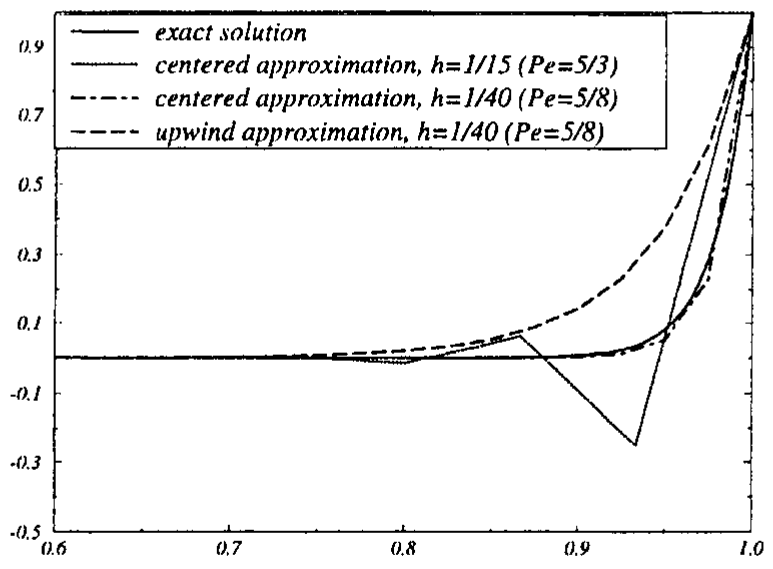
\includegraphics[width=.421\paperwidth]{images/fig-8-2-1.png}
  \caption{\(\varepsilon=1/50\)、\(b=1\) 时\eqref{eq:8.2.1}的精确解、中心差分逼近和迎风差分逼近}\label{fig:8.2.1}
\end{figure}

因此可以先得出如下结论：若对流--扩散问题存在边界层,且网格尺寸 \(h\) 大于 \(2\varepsilon/b\),Galerkin 解就可能出现振荡.第~\BookRef{sec:8.3}{8.3}~节将介绍如何克服这一困难.

线性方程组\eqref{eq:8.2.2}与用\emph{中心有限差分}逼近\eqref{eq:8.2.1}所得的方程组等价.这里之所以一致,是因为采用了均匀网格,且对流速度 \(b\) 为常数.事实上,中心差分格式为
\begin{equation}\label{eq:8.2.8}
  \begin{cases}
    -\varepsilon\dfrac{u_{j+1}-2u_j+u_{j-1}}{h^2}
        +b\dfrac{u_{j+1}-u_{j-1}}{2h}=0,\quad j=1,\ldots,M-1,\\[6pt]
    u_0=0,\\
    u_M=1,
  \end{cases}
\end{equation}
其中 \(u_j\) 是 \(u(x_j)\) 的近似值.这是一组线性差分方程,其解为 \(u_j=\xi_j\),其中 \(\xi_j\) 由\eqref{eq:8.2.6}给出(例如,见\BookCite{isaacson-keller1966}{Isaacson 和 Keller(1966)}第 8.4 节).因此,采用分片线性多项式的 Galerkin 法与中心有限差分逼近等价.

\begin{note}\NumberedNote{note:8.2.1}
暂且离开问题\eqref{eq:8.2.1},考虑反应--扩散问题
\SourcePage{271}
\[
  \begin{cases}
    -\varepsilon D^2u+a_0u=0,\quad 0<x<1,\\
    u(0)=0,\\
    u(1)=1,
  \end{cases}
\]
其中 \(\varepsilon>0\)、\(a_0>0\).其解为
\[
  u(x)=\frac{\sinh(\sqrt{a_0/\varepsilon}\,x)}{\sinh(\sqrt{a_0/\varepsilon})}.
\]
只要 \(\varepsilon/a_0\) 足够小,解就在 \(x=1\) 附近有一个宽度为 \(O(\sqrt{\varepsilon/a_0})\) 的边界层.

中心有限差分格式用下式逼近精确解 \(u(x_j)\)：
\begin{equation}\label{eq:8.2.9}
  \xi_j=(\tau_2^M-\tau_1^M)^{-1}(\tau_2^j-\tau_1^j),\qquad j=1,\ldots,M-1,
\end{equation}
其中 \(\tau_1=1+\sigma-\sqrt{\sigma(2+\sigma)}\),\(\tau_2=1+\sigma+\sqrt{\sigma(2+\sigma)}\),且 \(\sigma:=a_0h^2/(2\varepsilon)\).由于对任意网格尺寸 \(h\) 都有 \(0<\tau_1<1<\tau_2\),序列 \(\xi_j\) 单调递增.因此,无论 \(h\) 取何值,这一有限差分格式都不会产生振荡.

另一方面,采用分片线性有限元 Galerkin 法逼近该反应--扩散问题,得到下列方程组：
\[
  \varepsilon\sum_{i=0}^M\xi_i\int_0^1D\varphi_iD\varphi_j
    +a_0\sum_{i=0}^M\xi_i\int_0^1\varphi_i\varphi_j=0,\qquad j=1,\ldots,M-1,
\]
其中 \(\varphi_i\) 是包含端点的节点基函数,且 \(\xi_0=0\)、\(\xi_M=1\).算出积分后,得到代数方程组
\[
  \begin{cases}
    -\varepsilon\dfrac{\xi_{j+1}-2\xi_j+\xi_{j-1}}h
       +a_0h\dfrac{\xi_{j+1}+4\xi_j+\xi_{j-1}}6=0,\quad j=1,\ldots,M-1,\\[6pt]
    \xi_0=0,\\
    \xi_M=1.
  \end{cases}
\]
当 \(\sigma\ne3\) 时,相应的解形如\eqref{eq:8.2.9},但其中
\[
  \tau_1=\frac{3+2\sigma-\sqrt{3\sigma(\sigma+6)}}{3-\sigma},\qquad
  \tau_2=\frac{3+2\sigma+\sqrt{3\sigma(\sigma+6)}}{3-\sigma}.
\]
这两个特征根的符号都与 \(3-\sigma\) 相同.因此,当 \(\sigma>3\),即 \(h>\sqrt{6\varepsilon/a_0}\) 时,有限元解会出现振荡.

这一次,导致数值振荡的是零阶项 \(a_0u\).事实上,质量矩阵 \(M_{ij}:=\int_0^1\varphi_i\varphi_j\) 是恒等算子在有限元下的表示.若将它换成{\heiti 集中质量矩阵} \(\widehat M_{ij}:=(\sum_{k=0}^M M_{ik})\delta_{ij}\),可以立即验证,内点上的集中质量矩阵为 \(\widehat M=hI\).将内点方程除以 \(h\),就恰好得到有限差分格式,从而获得无条件稳定的解.关于时间依赖问题中的质量集中处理,见第~\BookRef{sec:11.4}{11.4}~节.\hfill\(\square\)
\end{note}

\subsection{迎风有限差分与数值扩散}\label{sec:8.2.2}
\SourcePage{272}

注意,问题\eqref{eq:8.2.1}中 \(b>0\),输运由左向右.因此,可以考虑用向后(\emph{迎风})有限差分逼近 \(bDu\).

所得格式可写为
\begin{equation}\label{eq:8.2.10}
  \begin{cases}
    -\varepsilon\dfrac{\widetilde u_{j+1}-2\widetilde u_j+\widetilde u_{j-1}}{h^2}
       +b\dfrac{\widetilde u_j-\widetilde u_{j-1}}h=0,\quad j=1,\ldots,M-1,\\[6pt]
    \widetilde u_0=0,\\
    \widetilde u_M=1,
  \end{cases}
\end{equation}
其解为
\begin{equation}\label{eq:8.2.11}
  \widetilde u_j=\frac{(1+2\mathrm{Pe})^j-1}{(1+2\mathrm{Pe})^M-1},
    \qquad j=1,\ldots,M-1.
\end{equation}
这一次,\(\widetilde u_j\) 不再振荡.事实上,对任意正的 \(\varepsilon\)、\(b\) 和 \(h\),均有 \(1+2\mathrm{Pe}>1\),所以 \(\widetilde u_j\) 随 \(j\) 递增(见\figref{fig:8.2.1}).

可以看到,这一迎风格式引入的局部截断误差为 \(O(h)\),而中心差分格式的局部截断误差为 \(O(h^2)\).需要注意,分片线性有限元的误差在 \(H^1\) 范数下按 \(O(h)\) 衰减(见\eqref{eq:6.2.8}),在最大范数下却按 \(O(h^2)\) 衰减(见\BookCite{ciarlet1968}{Ciarlet(1968)}).这与前面所见的一致：对常系数一维边值问题,均匀网格上的分片线性有限元与中心有限差分一致.

迎风格式的精度较低,但当 Péclet 数 \(\mathrm{Pe}>1\) 时,确实更适合用来逼近\eqref{eq:8.2.1}的解.

也可以从另一个角度解释这一事实.对 \(Du\) 的迎风逼近可以写成
\[
  \frac{\widetilde u_j-\widetilde u_{j-1}}h
   =\frac{\widetilde u_{j+1}-\widetilde u_{j-1}}{2h}
    -\frac h2\frac{\widetilde u_{j+1}-2\widetilde u_j+\widetilde u_{j-1}}{h^2}.
\]
因此,它相当于对正则化算子 \(D-\tfrac h2D^2\) 作中心差分逼近.换言之,迎风逼近引入了数值耗散,可将其看作对人工黏性项 \(-\tfrac h2D^2u\) 的直接离散.这通常称为\emph{数值扩散}(或\emph{数值黏性}).这也从另一个角度说明了迎风差分格式为何只有一阶精度.

迎风差分格式可以解释为\eqref{eq:8.2.1}的 Petrov--Galerkin 逼近.在这种方法中,近似解与试验函数分别取自不同的空间,通常记为 \(W_h\) 和 \(V_h\).逼近\eqref{eq:8.2.1}时,\SourcePage{273}可取 \(W_h=X_h^1\cap H_0^1(0,1)\)；相应的仿射子空间 \(W_h^*=\{v_h\in X_h^1\mid v_h(0)=0,\ v_h(1)=1\}\) 负责满足非齐次 Dirichlet 条件.为定义试验函数空间 \(V_h\),考察分片二次函数
\begin{equation}\label{eq:8.2.12}
  \sigma_2(x):=
  \begin{cases}
    -3x(1+x),&-1\le x\le0,\\
    -3x(1-x),&0\le x\le1,\\
    0,&|x|\ge1.
  \end{cases}
\end{equation}
这样便可引入有限维空间
\begin{equation}\label{eq:8.2.13}
  V_h=\operatorname{span}\{\psi_1,\ldots,\psi_{M-1}\},
\end{equation}
其中
\begin{equation}\label{eq:8.2.14}
  \psi_j(x):=\varphi_j(x)+\sigma_2(h^{-1}x-j),\qquad j=1,\ldots,M-1,
\end{equation}
而 \(\varphi_j\) 是 \(W_h\) 中与节点 \(x_j\) 对应的基函数.

容易验证(例如,见\BookCite{mitchell-griffiths1980}{Mitchell 和 Griffiths(1980)}第 221–223 页),\eqref{eq:8.2.10}对应的线性方程组与下列 Petrov--Galerkin 问题的方程组等价：
\[
  \text{求 }u_h\in W_h^*,\quad\text{使}\quad
  \int_0^1(\varepsilon Du_hDv_h+bDu_hv_h)=0\qquad\forall\,v_h\in V_h.
\]

\subsection{谱逼近}\label{sec:8.2.3}

本小节考察对流--扩散问题\eqref{eq:8.2.1}的 Chebyshev 配置逼近.可以看到,对流项占优时确实会出现振荡,但谱解仍满足某种形式的最大值原理.这些结果由\BookCite{canuto1988}{Canuto(1988)}给出.

为简便起见,在区间 \((-1,1)\) 上讨论与前面相同的 Dirichlet 问题,即
\begin{equation}\label{eq:8.2.15}
  \begin{cases}
    -\varepsilon D^2u+bDu=0,\quad -1<x<1,\\
    u(-1)=0,\\
    u(1)=1.
  \end{cases}
\end{equation}
对 \(N\ge2\),定义
\begin{equation}\label{eq:8.2.16}
  V_N^*:=\{v_N\in\mathbb P_N\mid v_N(-1)=0,\ v_N(1)=1\}
\end{equation}
及
\begin{equation}\label{eq:8.2.17}
  V_N=\mathbb P_N^0:=\{v_N\in\mathbb P_N\mid v_N(-1)=v_N(1)=0\},
\end{equation}
\SourcePage{274}则 Chebyshev 谱问题为
\begin{equation}\label{eq:8.2.18}
  \text{求 }u_N\in V_N^*,\quad\text{使}\quad
  \varepsilon\left(Du_N,\frac{D(v_Nw)}w\right)_N
       +b(Du_N,v_N)_N=0\qquad\forall\,v_N\in V_N,
\end{equation}
其中 \((\cdot,\cdot)_N\) 是\eqref{eq:4.2.4}中引入的离散内积,Chebyshev 节点和权重分别由\eqref{eq:4.3.12}和\eqref{eq:4.3.13}给出.

注意,\eqref{eq:8.2.18}同时体现了 Galerkin 法和配置法.事实上,由于 \(v_N=(1-x^2)p_{N-2}\),其中 \(p_{N-2}\in\mathbb P_{N-2}\),有 \(D(v_Nw)/w\in\mathbb P_{N-1}\).于是由\eqref{eq:4.2.6}可得
\[
  \left(Du_N,\frac{D(v_Nw)}w\right)_N
    =\left(Du_N,\frac{D(v_Nw)}w\right)_w
\]
和
\[
  (Du_N,v_N)_N=(Du_N,v_N)_w.
\]
因此,\eqref{eq:8.2.18}可以看成相对于内积 \((\cdot,\cdot)_w\) 的\eqref{eq:8.2.15}的 Galerkin 法.此外,由于
\[
  \left(Du_N,\frac{D(v_Nw)}w\right)_w
      =-(D^2u_N,v_N)_w=-(D^2u_N,v_N)_N
\]
(仍用了\eqref{eq:4.2.6}),可从\eqref{eq:8.2.18}推出 \(u_N\) 满足
\[
  -\varepsilon D^2u_N+bDu_N=0\qquad
  \text{在 }x_j=\cos\frac{\pi j}{N},\quad j=1,\ldots,N-1,
\]
即满足一个配置问题.

\eqref{eq:8.2.15}的精确解
\[
  u(x)=(e^{2b/\varepsilon}-1)^{-1}[e^{b(x+1)/\varepsilon}-1]
\]
是递增函数,且满足最大值原理 \(0\le u(x)\le1\).近似解 \(u_N(x)\) 则不一定满足这一性质,因为当 \(\varepsilon/b\) 远小于 \(1/N\) 时,\(x=1\) 附近会出现 Gibbs 现象.

换言之,谱配置逼近或谱 Galerkin 逼近在\emph{物理空间}中不满足最大值原理.不过,在\emph{频率空间}中可能有某种形式的最大值原理.事实上,可以证明谱解
\[
  u_N(x)=\sum_{m=0}^N\widehat u_mT_m(x)
\]
的 Chebyshev 系数满足 \(\widehat u_m>0\)(\(1\le m\le N\)),其中 \(T_m(x)\) 是\eqref{eq:4.3.2}中引入的 Chebyshev 多项式.

这一事实的一个重要推论是
\SourcePage{275}
\begin{equation}\label{eq:8.2.19}
  \begin{aligned}
  u_N(x)=\sum_{m=0}^N\widehat u_m T_m(x)
     &\le \widehat u_0+\sum_{m=1}^N\widehat u_m|T_m(x)|\\
     &\le\sum_{m=0}^N\widehat u_m
       =\sum_{m=0}^N\widehat u_mT_m(1)=u_N(1)=1
  \end{aligned}
\end{equation}
对任意 \(x\in[-1,1]\) 成立.因此,边界数据给出了 \(u_N(x)\) 的一致上界.

若 \(\varepsilon/b\) 与 \(1/N^2\) 相比足够小,即
\begin{equation}\label{eq:8.2.20}
  \frac{\varepsilon}{b}\le C_0N^{-2}
\end{equation}
对一个较小的常数 \(C_0>0\) 成立,则可得到更精确的结果.注意,此时 \(x=1\) 附近确实出现 Gibbs 现象.在这一情形下,若 \(N\) 为奇数,则 \(\widehat u_m>0\)(\(0\le m\le N\)).仿照\eqref{eq:8.2.19}的证明可得,对 \(-1\le x\le1\),有 \(|u_N(x)|\le1\).若 \(N\) 为偶数,则 \(\widehat u_0<0\),而 \(\widehat u_m>0\)(\(1\le m\le N\)),所以对 \(-1\le x\le1\) 有 \(-1-2|\widehat u_0|\le u_N(x)\le1\).不过,这时 \(|\widehat u_0|\) 依赖于 \(\varepsilon\)、\(b\) 和 \(N\),确切地说,它与 \(N^{-2}b/\varepsilon\) 同阶,因而 \(u_N(x)\) 没有一致下界.特别是,当 \(\varepsilon/b\) 远小于 \(1/N\) 时,这一结果表明,对流占优问题的谱逼近可能对 \(N\) 的奇偶性非常敏感.

\section{稳定化方法}\label{sec:8.3}

现在回到一般的 \(d\) 维问题
\begin{equation}\label{eq:8.3.1}
  \begin{cases}
    Lu=f,&\text{在 }\Omega\text{ 内},\\
    u=0,&\text{在 }\partial\Omega\text{ 上},
  \end{cases}
\end{equation}
其中 \(d=2,3\),\(L\) 由\eqref{eq:8.1.1}定义.为简便起见,取 \(\Omega\) 为多边形区域.

将\eqref{eq:8.3.1}写成\eqref{eq:8.1.7}的形式后,其 Galerkin 逼近为
\begin{equation}\label{eq:8.3.2}
  \text{求 }u_h\in V_h,\quad\text{使}\quad
    a(u_h,v_h)=(f,v_h)\qquad\forall\,v_h\in V_h,
\end{equation}
其中 \(V_h\) 是 \(V=H_0^1(\Omega)\) 的适当有限维子空间.上一节已经看到,若相对于 \(\|\boldsymbol{b}\|_{L^\infty(\Omega)}\) 与网格尺寸 \(h\) 的乘积而言,椭圆性常数 \(\alpha_0\) 很小,这一方法就可能无法给出令人满意的近似解.

\SourcePage{276}
\begin{example}[对流占优时 Galerkin 解的振荡]\label{ex:8.3-galerkin}
\figref{fig:8.3.1}给出一个实例.图中是对流--扩散方程
\begin{equation}\label{eq:8.3.3}
  -\varepsilon\Delta u+\operatorname{div}(\boldsymbol{b}u)=0
    \qquad\text{在 }\Omega=(0,1)^2\text{ 内}
\end{equation}
的分片线性有限元 Galerkin 逼近,其中 \(\varepsilon=10^{-3}\)、\(\boldsymbol{b}=(0,1)\),剖分采用 \(30\times30\) 个均匀分布的节点.可以清楚地看到,解在层的两侧出现严重振荡.
\end{example}

\begin{figure}[!htbp]
  \centering
  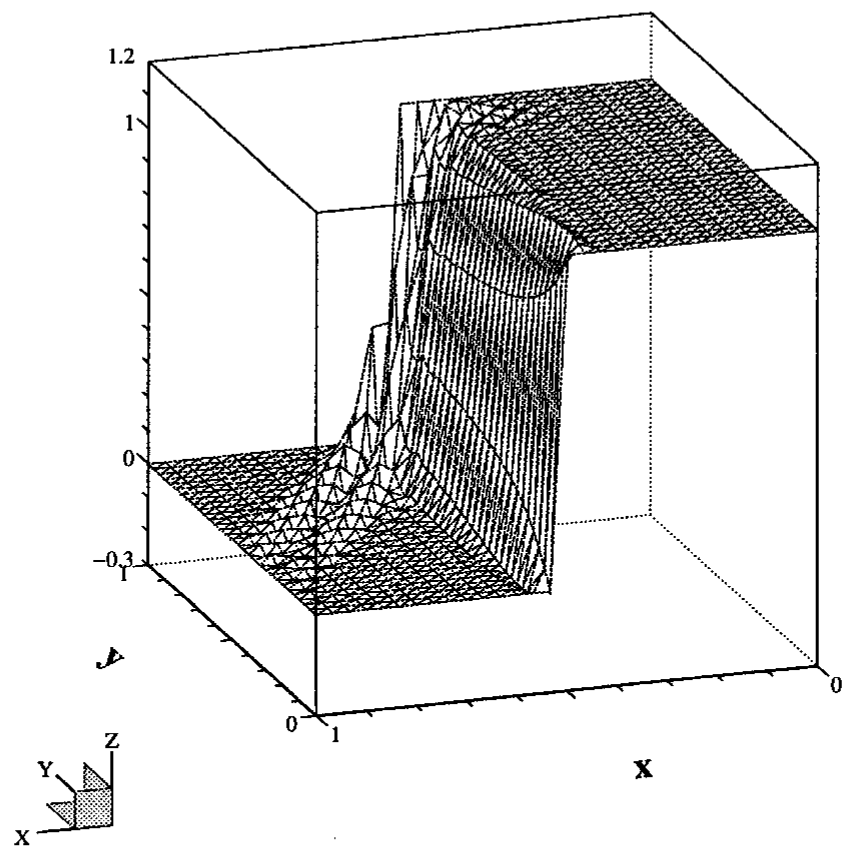
\includegraphics[width=.465\paperwidth]{images/fig-8-3-1.png}
  \caption{用 Galerkin 法得到的数值结果}\label{fig:8.3.1}
\end{figure}

注意,对于问题\eqref{eq:8.3.3},对流项对稳定性估计不起作用.因此,无法得到与参数 \(\varepsilon\) 无关的先验控制.

前面已经表明,一种可能的补救措施是采用 Petrov--Galerkin 逼近.在一维情形,它等价于迎风有限差分格式.不过,这种方法引入了 \(O(h)\) 量级的数值黏性,影响了逼近精度.

下面回顾几种用于逼近 \(d\) 维问题\eqref{eq:8.3.1}的方法.首先介绍具有一阶精度的人工扩散法,随后着重讨论几种具有强相容性(见\eqref{eq:8.3.6})和高阶精度的稳定化方法.

\subsection{人工扩散法}\label{sec:8.3.1}
\SourcePage{277}

经典的\emph{人工扩散法}是一维迎风有限差分格式在 \(d\) 维情形下的推广.它在所有方向上引入 \(O(h)\) 量级的数值扩散.

这一方法的思想很容易解释.Galerkin 法在 Péclet 数 \(\mathrm{Pe}\) 较大时会产生振荡,此时椭圆性常数 \(\alpha_0\) 相对于 \(\|\boldsymbol{b}\|_{L^\infty(\Omega)}\) 与 \(h\) 的乘积很小.为避免这一困难,可将原问题改为椭圆性常数更大的问题.例如,在 \(L\) 上加上算子 \(\mathcal L\),其中
\[
  \mathcal Lz:=-hQ\Delta z,\qquad Q:=\|\boldsymbol{b}\|_{L^\infty(\Omega)}.
\]
椭圆性常数变为 \(\alpha_0^*:=\alpha_0+hQ\).对新算子应用 Galerkin 法,得到不再受振荡影响的近似解.

新的解 \(u_h^*\) 满足
\begin{equation}\label{eq:8.3.4}
  u_h^*\in V_h:\quad a_h(u_h^*,v_h)=(f,v_h)\qquad\forall\,v_h\in V_h,
\end{equation}
其中
\[
  a_h(z,v):=a(z,v)+hQ(\nabla z,\nabla v)\qquad\forall\,z,v\in V.
\]
这是一个广义 Galerkin 问题(见第~\ref{sec:5.5}~节).

这种处理有一个明显的缺点.由于附加项 \(-hQ\Delta z\) 为 \(O(h)\) 量级,特别有
\begin{equation}\label{eq:8.3.5}
  \sup_{\substack{v_h\in V_h\\v_h\ne0}}
     \frac{|a_h(u,v_h)-(f,v_h)|}{\|v_h\|_1}=O(h),
\end{equation}
其中 \(u\) 是\eqref{eq:8.3.1}的解.这说明格式是\emph{相容}的,但只有一阶相容性.因此,无论有限元空间的多项式次数 \(k\) 有多高,人工扩散法的精度都不会超过一阶.

对于最低次的分片线性有限元(\(k=1\)),上述稳定化仍能保持误差 \(H^1\) 范数下的一阶精度,但会使误差的最大范数从 \(O(h^2|\log h|)\)(见笔记~\ref{note:6.2.3})退化到 \(O(h)\).

因此,稳定项与多项式逼近本来可以保证的最优阶不相容.采用谱方法时,精度损失更加明显.

应用命题~\ref{pro:5.5.1}可得到人工扩散法的误差估计.具体来说,
\[
  \|u-u_h^*\|_1\le C\left(\inf_{v_h\in V_h}\|u-v_h\|_1+h\|u\|_1\right),
\]
\SourcePage{278}其中 \(C=C(\alpha,\gamma,Q)\),而 \(\alpha\) 和 \(\gamma\) 分别是双线性形式 \(a(\cdot,\cdot)\) 的强制性常数和连续性常数.

和一维迎风有限差分的情形一样,稳定性的获得以精度损失为代价.典型结果会表现出过度扩散,\figref{fig:8.2.1}已经给出了一维的情形.在二维情形,除了沿流线方向(即与 \(\boldsymbol{b}(\boldsymbol{x})\) 方向平行的曲线方向)有扩散,在与之垂直的方向上也可观察到扩散.这种不希望出现的现象通常称为\emph{横风扩散},见\figref{fig:8.3.2}.

\begin{figure}[!htbp]
  \centering
  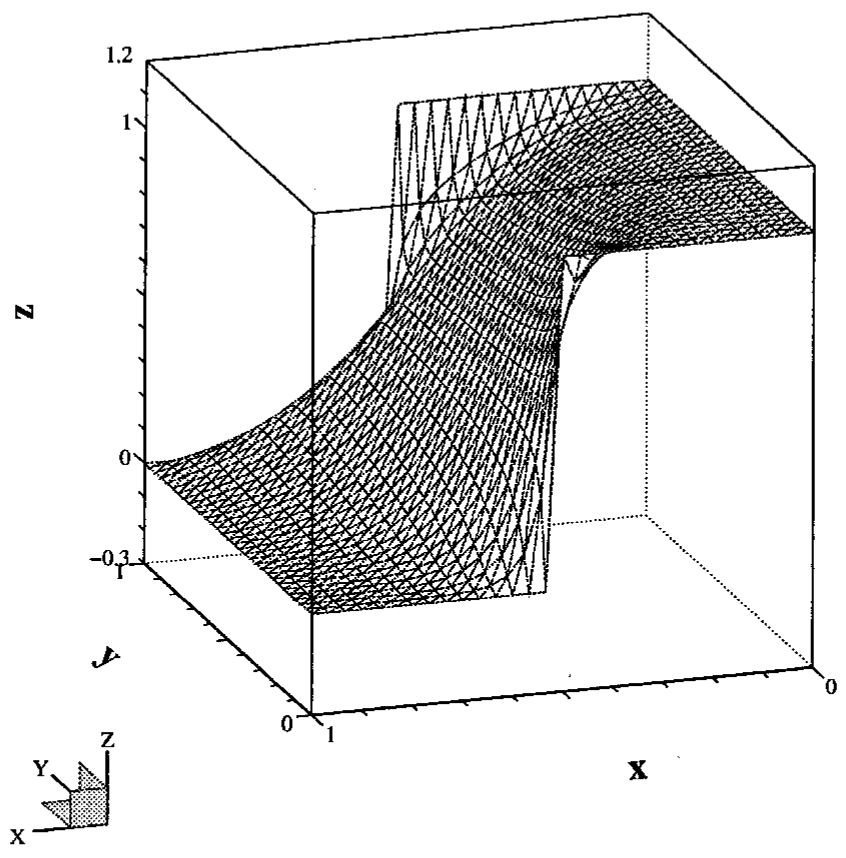
\includegraphics[width=.461\paperwidth]{images/fig-8-3-2.png}
  \caption{用人工扩散法得到的数值结果}\label{fig:8.3.2}
\end{figure}

可以在 \(L\) 上加上如下算子 \(\widehat{\mathcal L}\) 来避免横风扩散：
\[
  \widehat{\mathcal L}z:=-\frac hQ\operatorname{div}
       [(\boldsymbol{b}\cdot\nabla z)\boldsymbol{b}].
\]
它在 \(H_0^1(\Omega)\) 上不具有强制性,但满足
\[
  \int_\Omega(\widehat{\mathcal L}v)v=\frac hQ\int_\Omega(\boldsymbol{b}\cdot\nabla v)^2
    \ge0\qquad\forall\,v\in H_0^1(\Omega).
\]
这一做法称为\emph{流线迎风法}.在有限差分格式中由\BookCite{raithby1976}{Raithby(1976)}提出,在有限元框架下由\BookCite{hughes-brooks1979}{Hughes 和 Brooks(1979)}提出.它产生的人工扩散只沿流线方向影响近似解.\SourcePage{279}不过,它仍引入一阶附加项,所以只有 \(O(h)\) 精度.

\begin{note}\NumberedNote{note:8.3.1}
文献中还提出了其他几种迎风型有限元法.下一小节将介绍不同作者提出的一族稳定化方法.关于较早格式的理论介绍和计算效率分析,见\BookCite{ikeda1983}{Ikeda(1983)}、\BookCite{tabata1986}{Tabata(1986)}及其中所引文献.\hfill\(\square\)
\end{note}

\subsection{有限元的强相容稳定化方法}\label{sec:8.3.2}

本小节介绍几种能保持多项式子空间固有精度的稳定化方法.这些方法都属于\eqref{eq:5.5.1}所述的广义 Galerkin 法.若 \(u\) 是问题\eqref{eq:8.3.1}的精确解,则有
\begin{equation}\label{eq:8.3.6}
  \mathcal A_h(u,v_h)-\mathcal F_h(v_h)=0\qquad\forall\,v_h\in V_h.
\end{equation}
这个性质加强了相容性\eqref{eq:8.3.5},称为\emph{强相容性}.它使稳定化方法能够保持由有限维子空间的选取所决定的最优精度.

下面会看到,即使 Péclet 数很大,这些方法仍能给出无振荡的解.某些数值扩散依然存在,但主要沿流线方向影响解,使横风扩散明显减弱.

此外,适当调整这些方法,也可以用来处理其他问题中的不同类型的数值病态.例如,在 Stokes 问题的逼近中,不稳定性来自伪压力模态.若速度和压力的逼近子空间之间不满足适当的相容性条件,就可能出现这类模态(见第~\BookRef{sec:9.2}{9.2}~节和第~\BookRef{sec:9.4}{9.4}~节).

考察\eqref{eq:8.1.1}引入的算子 \(L\),按 \(L^2(\Omega)\) 的内积将它分解为对称部分和斜对称部分,即
\begin{equation}\label{eq:8.3.7}
  L=L_S+L_{SS},
\end{equation}
其中
\SourcePage{280}
\begin{align}
  L_S z&:=-\sum_{i,j=1}^d D_i(a_{ij}^S D_jz)
              +\left(\frac12\operatorname{div}\boldsymbol{b}+a_0\right)z,\label{eq:8.3.8}\\
  L_{SS} z&:=-\sum_{i,j=1}^d D_i(a_{ij}^{SS}D_jz)
        +\frac12\operatorname{div}(\boldsymbol{b}z)+\frac12\boldsymbol{b}\cdot\nabla z,\label{eq:8.3.9}
\end{align}
并且
\begin{equation}\label{eq:8.3.10}
  a_{ij}^S:=\frac{a_{ij}+a_{ji}}2,\qquad
  a_{ij}^{SS}:=\frac{a_{ij}-a_{ji}}2,\qquad i,j=1,\ldots,d.
\end{equation}

取 \(\overline\Omega\) 的一族正则剖分 \(\mathcal T_h\)(见定义~\ref{def:3.4.1}),并考察由分片光滑函数组成的有限维子空间 \(V_h\subset V=H_0^1(\Omega)\).例如,可以选取 \(V_h=X_h^k\cap H_0^1(\Omega)\)、\(k\ge1\),其中 \(X_h^k\) 是\eqref{eq:3.2.4}或\eqref{eq:3.2.5}定义的有限元空间.

本章讨论\emph{对流占优情形},即假设每个 \(K\in\mathcal T_h\) 上的局部 Péclet 函数 \(\mathrm{Pe}_K(\boldsymbol{x})\) 大于 \(1\)：
\begin{equation}\label{eq:8.3.11}
  \mathrm{Pe}_K(\boldsymbol{x}):=
    \frac{|\boldsymbol{b}(\boldsymbol{x})|h_K}{2\alpha_0(\boldsymbol{x})}>1
    \qquad\forall\,\boldsymbol{x}\in K,
\end{equation}
其中
\begin{equation}\label{eq:8.3.12}
  \alpha_0(\boldsymbol{x}):=\min_{\boldsymbol{\xi}\in\mathbb R^d\setminus\{0\}}
    \frac{\sum_{i,j=1}^d a_{ij}(\boldsymbol{x})\xi_i\xi_j}{|\boldsymbol{\xi}|^2},
      \qquad \boldsymbol{x}\in\overline\Omega.
\end{equation}
这里及下文均假设系数 \(a_{ij}(\boldsymbol{x})\) 和 \(\boldsymbol{b}(\boldsymbol{x})\) 在 \(\overline\Omega\) 上连续.注意,由椭圆性假设(见定义~\ref{def:6.1.1}),对于每个 \(\boldsymbol{x}\in\overline\Omega\),都有 \(\alpha_0(\boldsymbol{x})\ge\alpha_0>0\).此外,\eqref{eq:8.3.11}特别蕴含 \(\inf_\Omega|\boldsymbol{b}(\boldsymbol{x})|>0\).

现在可以引入\eqref{eq:8.3.1}的\emph{稳定化逼近}.定义
\[
  \begin{aligned}
    \mathcal L_h^{(\rho)}(z_h,v_h)
      &:=\sum_{K\in\mathcal T_h}\delta\left(
           Lz_h,\frac{h_K}{|\boldsymbol{b}|}(L_{SS}+\rho L_S)v_h\right)_K,\\
    \varphi_h^{(\rho)}(v_h)
      &:=\sum_{K\in\mathcal T_h}\delta\left(
           f,\frac{h_K}{|\boldsymbol{b}|}(L_{SS}+\rho L_S)v_h\right)_K,
  \end{aligned}
\]
其中 \(z_h,v_h\in V_h\),\((\cdot,\cdot)_K\) 表示 \(L^2(K)\) 的内积,参数 \(\delta>0\) 和 \(\rho\in\mathbb R\) 有待选定.于是,考虑如下问题：
\begin{equation}\label{eq:8.3.13}
  \text{求 }u_h\in V_h,\quad\text{使}\quad
     a(u_h,v_h)+\mathcal L_h^{(\rho)}(u_h,v_h)
       =(f,v_h)+\varphi_h^{(\rho)}(v_h)\qquad\forall\,v_h\in V_h.
\end{equation}
进一步,用 \(a_h^{(\rho)}(\cdot,\cdot)\) 表示上面的稳定化双线性形式,即
\SourcePage{281}
\begin{equation}\label{eq:8.3.14}
  a_h^{(\rho)}(z_h,v_h):=a(z_h,v_h)+\mathcal L_h^{(\rho)}(z_h,v_h)
     \qquad\forall\,z_h,v_h\in V_h,
\end{equation}
用 \(\mathcal F_h^{(\rho)}(\cdot)\) 表示经扰动的连续线性泛函
\[
  \mathcal F_h^{(\rho)}(v_h):=(f,v_h)+\varphi_h^{(\rho)}(v_h)\qquad\forall\,v_h\in V_h.
\]

先说明一个重要的事实.由于精确解 \(u\) 满足 \(Lu=f\in L^2(\Omega)\),对每个 \(v_h\in V_h\),\(a_h^{(\rho)}(u,v_h)\) 都有定义.此外,无论怎样选取 \(\delta\) 和 \(\rho\),问题\eqref{eq:8.3.13}都具有\eqref{eq:8.3.6}意义下的\emph{强相容性}.现在的问题是如何选取合适的参数,使得在适当范数下同时具有稳定性和收敛性.

第~\BookRef{sec:8.4}{8.4}~节将分析参数 \(\rho\) 取三个不同值时的稳定化问题\eqref{eq:8.3.13}.这些方法分别由不同的研究者提出.这里沿用\BookCite{baiocchi-brezzi1992}{Baiocchi 和 Brezzi(1992)}的做法,将它们放在统一的框架下介绍.\(\rho=0\) 对应 \emph{SUPG 法(流线迎风/Petrov--Galerkin 法)},由\BookCite{hughes-brooks1982}{Hughes 和 Brooks(1982)}及\BookCite{brooks-hughes1982}{Brooks 和 Hughes(1982)}提出.这一方法也称为\emph{流线扩散法},例如见\BookCite{johnson1987}{Johnson(1987)}.\(\rho=1\) 对应 \emph{GALS 法(Galerkin/最小二乘法)},由\BookCite{hughes-franca-hulbert1989}{Hughes、Franca 和 Hulbert(1989)}引入.\(\rho=-1\) 对应\BookCite{franca-frey-hughes1992}{Franca、Frey 和 Hughes(1992)}提出的方法,它将\BookCite{douglas-wang1989}{Douglas 和 Wang(1989)}在 Stokes 问题逼近中使用的思想推广到对流--扩散方程.称最后这一种为 \emph{DWG 法(Douglas--Wang/Galerkin 法)}.应当注意,当扩散系数在各单元上为常数、\(\tfrac12\operatorname{div}\boldsymbol{b}+a_0=0\) 且以分片线性多项式作为试验函数时,上述三种方法一致.

\begin{note}\NumberedNote{note:8.3.2}
如前所述,SUPG 是流线迎风/Petrov--Galerkin 的缩写.不过,正如\BookCite{hughes1987}{Hughes(1987)}指出的,这一名称未必恰当.实际上,SUPG 是\eqref{eq:8.3.13}的特例,而\eqref{eq:8.3.13}是广义 Galerkin 法.\hfill\(\square\)
\end{note}

\begin{note}\NumberedNote{note:8.3.3}
在{\heiti 扩散占优情形},即对每个 \(K\in\mathcal T_h\) 和每个 \(\boldsymbol{x}\in K\) 都有 \(\mathrm{Pe}_K(\boldsymbol{x})\le1\) 时,标准 Galerkin 法就能令人满意地处理这一问题.不过,只要将稳定化参数 \(\delta\) 取为 \(\mathrm{Pe}_K\) 的函数,具体取 \(\delta=O(\mathrm{Pe}_K)\),也可使用\eqref{eq:8.3.13}的稳定化方法(另见笔记~\BookRef{note:8.4.2}{8.4.2}).\hfill\(\square\)
\end{note}

最后给出一些数值结果.先用稳定化 GALS 法和分片二次有限元逼近对流--扩散方程\eqref{eq:8.3.3},其中取 \(\varepsilon=10^{-5}\).剖分采用 \(30\times30\) 个均匀分布的节点.选取几种不同的对流场 \(\boldsymbol{b}\) 和 \(u\) 的边界值.每个算例中的\SourcePage{282}\(\boldsymbol{b}\) 及边界数据都可以直接从下面的图中看出.\figref{fig:8.3.3}\subref{fig:8.3.3a} 和 \subref{fig:8.3.3b} 表明,数值耗散只能沿流线方向增加.图 \subref{fig:8.3.3a} 中完全没有耗散,图 \subref{fig:8.3.3b} 中则由于流线穿过间断线而出现扩散.后一情形下还可看到一些欠冲和过冲,这在此类稳定化方法中时常发生(另见\figref{fig:8.3.3}\subref{fig:8.3.3c}).图 \subref{fig:8.3.3c} 和 \subref{fig:8.3.3d} 对应的测试问题实际上相同.不过,图 \subref{fig:8.3.3d} 表明,网格取向可能产生显著影响,导致即使 \(\boldsymbol{b}\) 与间断线平行,也出现数值扩散.

层附近出现的欠冲与过冲说明格式缺乏单调性.可在\eqref{eq:8.3.13}中再引入一个稳定项来克服这一缺陷.所加的是一个激波捕捉型非线性黏性项,见\BookCite{hughes-mallet-mizukami1986}{Hughes、Mallet 和 Mizukami(1986)}、\BookCite{galeao-dutradocarmo1988}{Galeão 和 Dutra do Carmo(1988)}、\BookCite{shakib1988}{Shakib(1988)}.

\begin{figure}[!htbp]
  \centering
  \caption{用 GALS 法得到的数值结果}\label{fig:8.3.3}
  \begin{subfigure}{\linewidth}
    \centering
    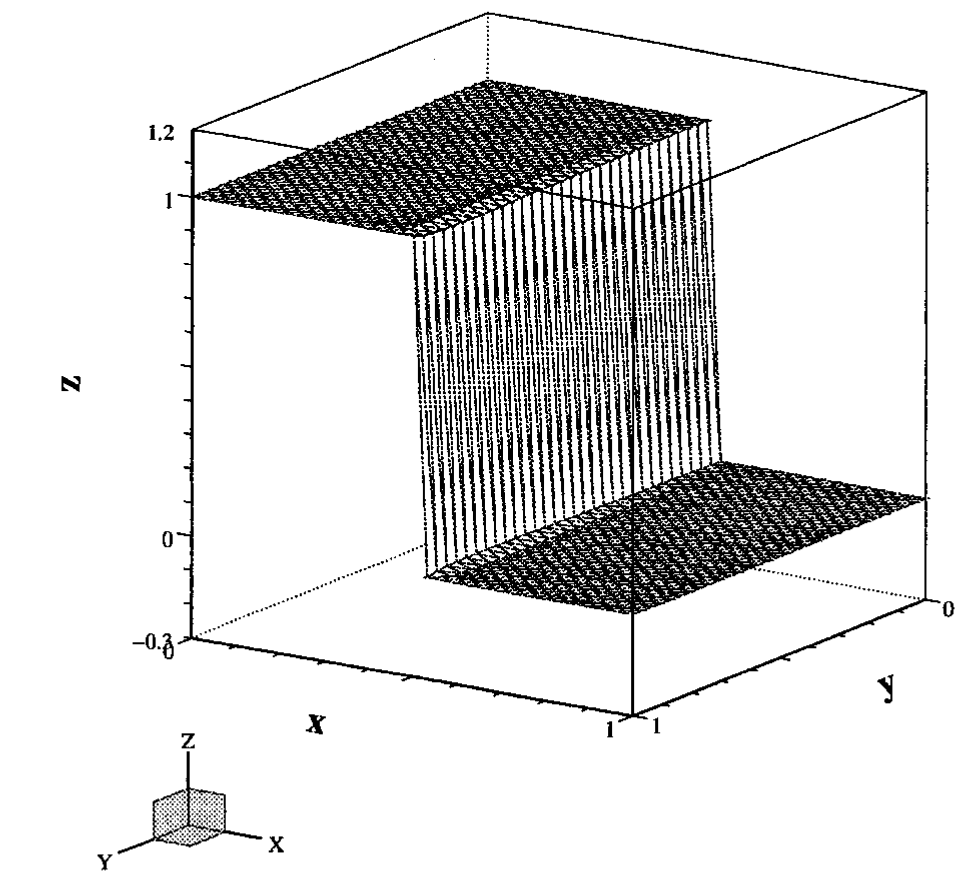
\includegraphics[width=.527\paperwidth]{images/fig-8-3-3a.png}
    \caption{}\label{fig:8.3.3a}
  \end{subfigure}\par\medskip
  \begin{subfigure}{\linewidth}
    \centering
    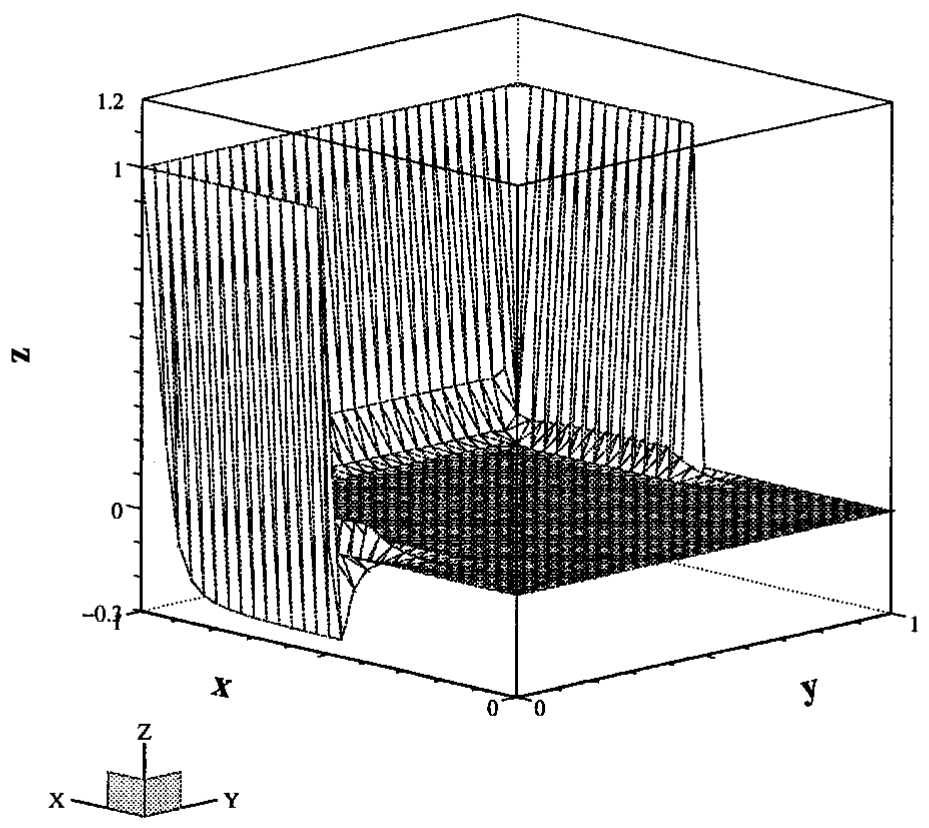
\includegraphics[width=.507\paperwidth]{images/fig-8-3-3b.png}
    \caption{}\label{fig:8.3.3b}
  \end{subfigure}
\end{figure}
\begin{figure}[!htbp]
  \ContinuedFloat
  \centering
  \caption[]{用 GALS 法得到的数值结果(续)}
  \begin{subfigure}{\linewidth}
    \centering
    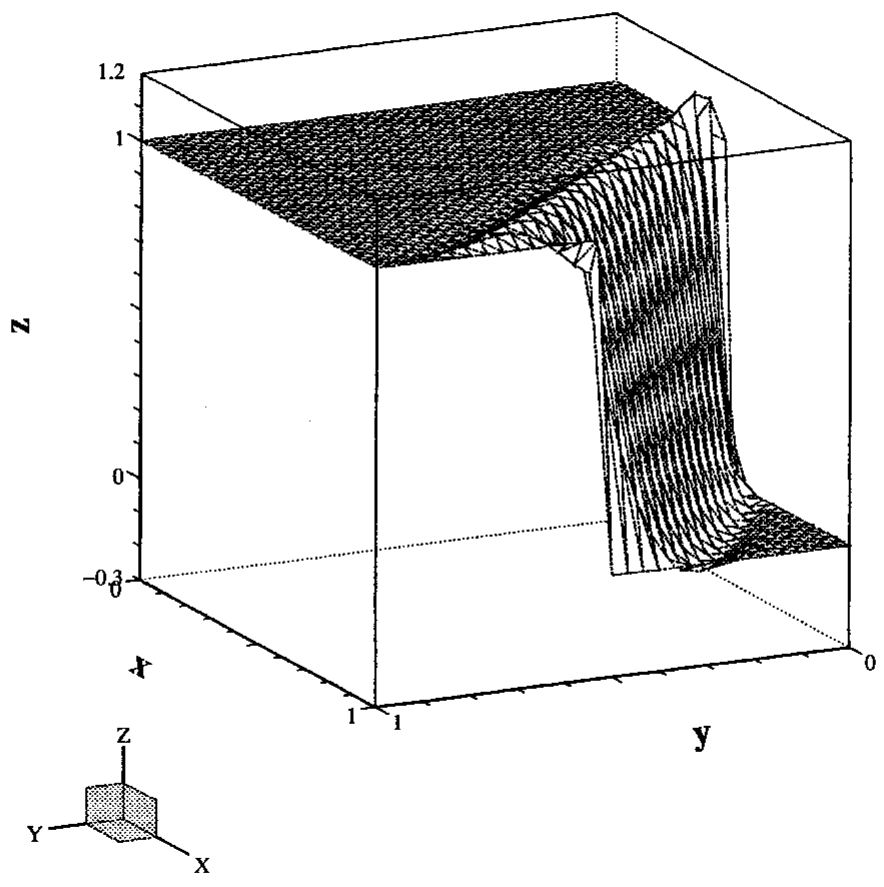
\includegraphics[width=.483\paperwidth]{images/fig-8-3-3c.png}
    \caption{}\label{fig:8.3.3c}
  \end{subfigure}\par\medskip
  \begin{subfigure}{\linewidth}
    \centering
    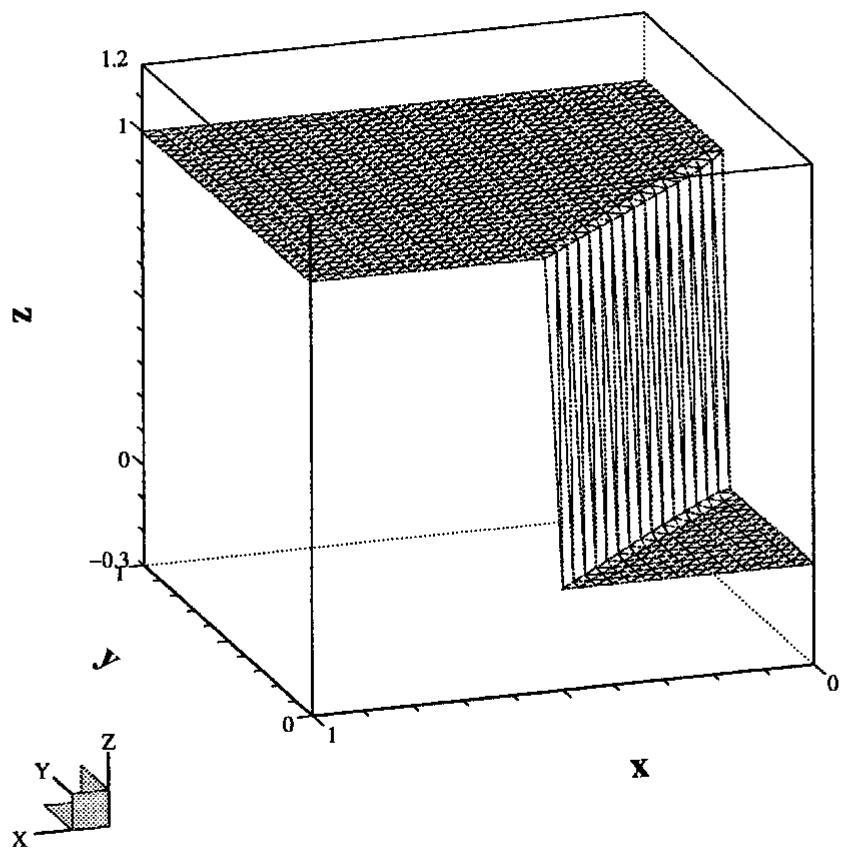
\includegraphics[width=.461\paperwidth]{images/fig-8-3-3d.png}
    \caption{}\label{fig:8.3.3d}
  \end{subfigure}
\end{figure}

\clearpage
\subsection{利用泡函数稳定化}\label{sec:8.3.3}
\SourcePage{283}

在分析上一小节所给方法的稳定性和收敛性之前,先介绍另一种解释.最早的解释由\BookCite{brezzi-bristeau-franca-mallet-roge1992}{Brezzi、Bristeau、Franca、Mallet 和 Rogé(1992)}给出.进一步的说明和改进见\BookCite{baiocchi-brezzi-franca1993}{Baiocchi、Brezzi 和 Franca(1993)}.关于不同背景下的类似方法,另见笔记~\BookRef{note:9.4.2}{9.4.2}.

为简便起见,仅考虑二维情形,即 \(d=2\).先引入有限维空间
\begin{equation}\label{eq:8.3.15}
  V_h^b:=[X_h^k\cap H_0^1(\Omega)]\oplus B,
\end{equation}
其中 \(X_h^k\) 按\eqref{eq:3.2.4}定义,\(B\) 是由\emph{泡函数}组成的有限维空间,在每个单元 \(K\in\mathcal T_h\) 上恰有一个自由度.例如,若 \(k<3\),可以选用三次泡函数,即
\begin{equation}\label{eq:8.3.16}
  B=B_3:=\{v_B\in H_0^1(\Omega)\mid
       v_B|_K=c_Kb_K,\ c_K\in\mathbb R,\ b_K=\lambda_1\lambda_2\lambda_3
       \quad\forall\,K\in\mathcal T_h\}.
\end{equation}
这里的 \(\lambda_i\)(\(i=1,2,3\))为线性多项式,各自在 \(K\) 的一条边上为零,并在对顶点取值 \(1\).因此,泡函数的一个例子 \(b_K\) 在 \(K\) 的内部为正,在 \(\partial K\) 上为零.

现在考察\eqref{eq:8.3.1}在 \(V_h^b\) 中的 Galerkin 逼近：
\SourcePage{284}
\begin{equation}\label{eq:8.3.17}
  \begin{aligned}
    \text{求 }u_h+u_B\in V_h^b,\quad\text{使}\quad
      a(u_h+u_B,v_h+v_B)&=(f,v_h+v_B)\\
      &\qquad\forall\,v_h+v_B\in V_h^b.
  \end{aligned}
\end{equation}
我们想先求出 \(u_B\),再将\eqref{eq:8.3.17}改写成 \(X_h^k\cap H_0^1(\Omega)\) 中的稳定化 Galerkin 法.首先,在每个 \(K\) 上可以将 \(u_B\) 写成
\begin{equation}\label{eq:8.3.18}
  u_B|_K=c_{b,K}b_K.
\end{equation}
在\eqref{eq:8.3.17}中,选试验函数 \(v_h=0\) 和 \(v_B\in B\),其中
\[
  v_B=
  \begin{cases}
    b_K,&\text{在 }K\text{ 内},\\
    0,&\text{在 }\Omega\setminus K\text{ 上},
  \end{cases}
\]
便有
\[
  a(u_h+u_B,v_B)=a_K(u_h+c_{b,K}b_K,b_K),
\]
其中 \(a_K(\cdot,\cdot)\) 表示 \(a(\cdot,\cdot)\) 在三角形 \(K\) 上的限制.于是,\eqref{eq:8.3.17}成为
\[
  a_K(u_h,b_K)+c_{b,K}a_K(b_K,b_K)=(f,b_K)_K.
\]
由于 \(u_h|_K\) 是多项式且 \(b_K\) 在 \(\partial K\) 上为零,可以对第一项分部积分,得到
\begin{equation}\label{eq:8.3.19}
  c_{b,K}=\frac{(f-Lu_h,b_K)_K}{a_K(b_K,b_K)}.
\end{equation}

\SourcePage{285}现在在\eqref{eq:8.3.17}中选任意 \(v_h\in X_h^k\cap H_0^1(\Omega)\) 和 \(v_B=0\) 作为试验函数,得到
\[
  a(u_h,v_h)+\sum_{K\in\mathcal T_h}c_{b,K}a_K(b_K,v_h)=(f,v_h).
\]
分部积分后,\(a_K(b_K,v_h)\) 一项给出
\[
  a_K(b_K,v_h)=(b_K,L_Sv_h-L_{SS}v_h)_K
\]
(记号见\eqref{eq:8.3.8}和\eqref{eq:8.3.9}).同理,
\[
  a_K(b_K,b_K)=(L_Sb_K,b_K)_K.
\]
利用\eqref{eq:8.3.19},最终可将\eqref{eq:8.3.17}写成
\begin{equation}\label{eq:8.3.20}
  a(u_h,v_h)+a_B(f;u_h,v_h)=(f,v_h)\qquad\forall\,v_h\in X_h^k\cap H_0^1(\Omega),
\end{equation}
其中
\begin{equation}\label{eq:8.3.21}
  a_B(f;u_h,v_h):=\sum_{K\in\mathcal T_h}
      \frac{(Lu_h-f,b_K)_K(L_{SS}v_h-L_Sv_h,b_K)_K}{(L_Sb_K,b_K)_K}.
\end{equation}
\eqref{eq:8.3.1}的这一有限维逼近具有强相容性.与通常的 Galerkin 逼近相比,它多出附加项 \(a_B(f;u_h,v_h)\).此外,它与\eqref{eq:8.3.13}中 \(\rho=-1\) 时的 DWG 法相似,因为 DWG 法的附加项形如
\SourcePage{286}
\begin{equation}\label{eq:8.3.22}
  \sum_{K\in\mathcal T_h}\delta\left(
     Lu_h-f,\frac{h_K}{|\boldsymbol{b}|}(L_{SS}v_h-L_Sv_h)\right)_K.
\end{equation}

下面说明,至少在一种简化情形下,可以将\eqref{eq:8.3.21}写成\eqref{eq:8.3.22}的形式.取\eqref{eq:3.2.4}中的分片线性有限元(\(k=1\)).假设 \(\boldsymbol{b}(\boldsymbol{x})\) 为常向量、\(f(\boldsymbol{x})\) 为常数、\(a_0(\boldsymbol{x})=0\),且 \(a_{ij}(\boldsymbol{x})=\varepsilon\delta_{ij}\),其中 \(\varepsilon>0\) 为常数,\(\delta_{ij}\) 是 Kronecker 符号.这时,
\[
  L_Sz=-\varepsilon\Delta z,\qquad L_{SS}z=\boldsymbol{b}\cdot\nabla z,
\]
SUPG、GALS 和 DWG 法均一致.再按\eqref{eq:8.3.16}选取泡函数空间 \(B\).注意,泡函数 \(b_K\) 满足
\begin{equation}\label{eq:8.3.23}
  \int_Kb_K=C_1\operatorname{meas}(K)=C_{1,K}h_K^2,\qquad
    \int_K|\nabla b_K|^2=C_{2,K},
\end{equation}
其中常数 \(C_{1,K}\) 和 \(C_{2,K}\) 与 \(h_K\) 无关.

先计算 \((Lu_h-f,b_K)_K\).回顾 \(u_h|_K\in\mathbb P_1\),由\eqref{eq:8.3.23}有
\[
  \begin{aligned}
    (Lu_h-f,b_K)_K
      &=(\boldsymbol{b}\cdot\nabla u_h-f,b_K)_K
       =(\boldsymbol{b}\cdot\nabla u_h|_K-f)\int_K b_K\\
      &=(\boldsymbol{b}\cdot\nabla u_h|_K-f)C_{1,K}h_K^2.
  \end{aligned}
\]
同样,
\[
  (L_{SS}v_h-L_Sv_h,b_K)_K=(\boldsymbol{b}\cdot\nabla v_h,b_K)_K
    =(\boldsymbol{b}\cdot\nabla v_h|_K)C_1\operatorname{meas}(K).
\]
最后,由\eqref{eq:8.3.23}得
\[
  (L_Sb_K,b_K)_K=-\varepsilon(\Delta b_K,b_K)_K=\varepsilon C_{2,K}.
\]
因此可写成
\[
  \begin{aligned}
    a_B(f;u_h,v_h)
      &=\sum_{K\in\mathcal T_h}
        \frac{(\boldsymbol{b}\cdot\nabla u_h|_K-f)(\boldsymbol{b}\cdot\nabla v_h|_K)
             C_1C_{1,K}h_K^2\operatorname{meas}(K)}{\varepsilon C_{2,K}}\\
      &=\sum_{K\in\mathcal T_h}
        \frac{C_1C_{1,K}h_K^2}{\varepsilon C_{2,K}}(L_{SS}u_h-f,L_{SS}v_h)_K.
  \end{aligned}
\]
再由定义\eqref{eq:8.3.11}最终得到
\begin{equation}\label{eq:8.3.24}
  a_B(f;u_h,v_h)=\sum_{K\in\mathcal T_h}\frac{2C_1C_{1,K}\mathrm{Pe}_K}{C_{2,K}}
      \left(Lu_h-f,\frac{h_K}{|\boldsymbol{b}|}(L_{SS}v_h-L_Sv_h)\right)_K.
\end{equation}

\SourcePage{287}与\eqref{eq:8.3.13}比较便可看出,泡函数带来的附加项恰好是 DWG 法的稳定项,其中在每个单元 \(K\in\mathcal T_h\) 上适当选取常数 \(\delta=\delta_K\).再次注意,在当前假设下,\(L_Su_h=L_Sv_h=0\),所以 SUPG、GALS 和 DWG 法一致.

实际上,\eqref{eq:8.3.24}用于对流占优问题的逼近时还不够理想,因为常数 \(\delta_K:=2C_{2,K}^{-1}C_1C_{1,K}\mathrm{Pe}_K\) 依赖于局部 Péclet 数.不过,稍稍改变做法并选用其他类型的泡函数,就能得到形式\eqref{eq:8.3.13},其中参数 \(\delta_K\) 与 \(\mathrm{Pe}_K\) 无关.见\BookCite{brezzi-bristeau-franca-mallet-roge1992}{Brezzi、Bristeau、Franca、Mallet 和 Rogé(1992)}.

\subsection{谱逼近的稳定化方法}\label{sec:8.3.4}

本小节考察谱配置逼近的两种稳定化方法.第一种方法表明,在标准谱配置格式中增加具有局部支集的近似解基函数和试验函数(通常为泡函数),可以使格式稳定.第二种方法将第~\ref{sec:8.3.2}~节的方法推广到谱配置,在通常的 Galerkin 方法中加入与 SUPG、GALS 或 DWG 法类似的附加项.

为简便起见,集中讨论二维齐次 Dirichlet 问题
\begin{equation}\label{eq:8.3.25}
  \begin{cases}
    Lu:=-\varepsilon\Delta u+\operatorname{div}(\boldsymbol{b}u)+a_0u=f,
       &\text{在 }\Omega\text{ 内},\\
    u=0,&\text{在 }\partial\Omega\text{ 上},
  \end{cases}
\end{equation}
其中 \(f\in L^2(\Omega)\)、\(\Omega=(-1,1)^2\).与\eqref{eq:8.3.25}对应的双线性形式 \(a(\cdot,\cdot)\) 按\eqref{eq:8.1.2}定义,其中 \(a_{ij}=\varepsilon\delta_{ij}\).假设它连续且具有强制性,即满足\eqref{eq:8.1.3}和\eqref{eq:8.1.4}.相应的变分问题为
\begin{equation}\label{eq:8.3.26}
  \text{求 }u\in H_0^1(\Omega),\quad\text{使}\quad
    a(u,v)=(f,v)\qquad\forall\,v\in H_0^1(\Omega).
\end{equation}

对每个整数 \(N\ge2\),Legendre--Gauss--Lobatto 节点 \(\boldsymbol{x}_{ij}=(x_i,x_j)\)(\(i,j=0,\ldots,N\))诱导 \(\overline\Omega\) 的一个剖分 \(\mathcal T_h\),由 \(N^2\) 个矩形单元 \(K_{ij}:=I_i\times I_j\) 组成.每个单元的顶点是 Gauss--Lobatto 网格上的四个相邻节点.这里取 \(I_i:=[x_{i+1},x_i]\),因为 Legendre 节点通常从右向左排序,见第~\ref{sec:4.4.2}~节.仍以 \(w_{ij}\) 记 Legendre--Gauss--Lobatto 求积公式的权重(见\eqref{eq:4.5.38}).

令 \(V_N:=\mathbb Q_N^0\) 为每个变量 \(x\)、\(y\) 的次数均不超过 \(N\)、且在 \(\partial\Omega\) 上为零的多项式空间.类似地,令 \(V_h\) 为有限元空间 \(X_h^1\cap H_0^1(\Omega)\),其中 \(X_h^1\) 按\eqref{eq:3.2.5}定义.泡函数空间记为
\SourcePage{288}
\begin{equation}\label{eq:8.3.27}
  B:=\{v_B\in H_0^1(\Omega)\mid v_B|_{K_{ij}}=c_{ij}b_{ij},\
          c_{ij}\in\mathbb R,\ i,j=0,\ldots,N-1\},
\end{equation}
其中对每个 \(i,j\),预先选定一个在 \(K_{ij}\) 的边界上为零的函数 \(b_{ij}\).最简单的例子是 \(b_{ij}\in\mathbb Q_2\)、\(b_{ij}(x,y)=p_i(x)p_j(y)\),这里 \(p_i\) 和 \(p_j\) 是两个二次多项式,分别在区间 \(I_i\) 和 \(I_j\) 的两个端点处为零,在中点取值 \(1\).下文的\eqref{eq:8.3.33}给出一个更有用的选择.

沿用\BookCite{canuto1994}{Canuto(1994)}的做法,定义
\begin{equation}\label{eq:8.3.28}
  V_N^b:=V_N\oplus B,
\end{equation}
并引入\eqref{eq:8.3.26}在 \(V_N^b\) 中的 Galerkin 逼近：
\begin{equation}\label{eq:8.3.29}
  \text{求 }u_N^b\in V_N^b,\quad\text{使}\quad
    a(u_N^b,v_N^b)=(f,v_N^b)\qquad\forall\,v_N^b\in V_N^b.
\end{equation}
显然,该问题有唯一解 \(u_N^b\),且满足
\begin{align}
  \|u_N^b\|_1&\le\frac1\alpha\|f\|_0\qquad\forall\,N\ge2,\label{eq:8.3.30}\\
  \|u-u_N^b\|_1&\le\frac{\gamma}{\alpha}\inf_{v_N^b\in V_N^b}\|u-v_N^b\|_1
      \le\frac{\gamma}{\alpha}\inf_{v_N\in V_N}\|u-v_N\|_1,\label{eq:8.3.31}
\end{align}
因为 \(V_N\subset V_N^b\).这表明,该 Galerkin 逼近的先验误差界至少不劣于在 \(V_N\) 中使用标准 Galerkin 法所得的误差界.

不过,我们已经指出,谱 Galerkin 法难以实现(见第~\ref{sec:6.2.1}~节).因此,这里更关心如何给出\eqref{eq:8.3.26}的谱配置逼近.为此,假设 \(f\in C^0(\overline\Omega)\).为简便起见,再令 \(\boldsymbol{b}\) 为常向量且 \(a_0=a_0(\boldsymbol{x})\ge0\).

\BookCite{canuto1994}{Canuto(1994)}提出如下带泡函数修正的谱配置法：求 \(u_N^b=u_N+u_b\in V_N^b\),使
\begin{equation}\label{eq:8.3.32}
  \left\{
  \begin{aligned}
    (Lu_N,v_N)_N+a(u_b,\pi_h^1(v_N))
      &=(f,v_N)_N&&\forall\,v_N\in V_N,\\
    (\pi_h^1(Lu_N),v_b)+a(u_b,v_b)
      &=(\pi_h^1(f),v_b)&&\forall\,v_b\in B.
  \end{aligned}
  \right.
\end{equation}
这里,\((\cdot,\cdot)_N\) 是\eqref{eq:4.5.39}中引入的离散内积,\(\pi_h^1\colon C^0(\overline\Omega)\to X_h^1\) 是\eqref{eq:3.4.1}定义的有限元插值算子.

可以如下理解\eqref{eq:8.3.32}的由来.先按分解\eqref{eq:8.3.28}将\eqref{eq:8.3.29}分成两组方程,一组用试验函数 \(v_N\) 求 \(u_N\),另一组用试验函数 \(v_b\) 求 \(u_b\).然后,用基于 \((\cdot,\cdot)_N\) 的离散形式分别代替双线性形式 \(a(u_N,v_N)\) 和项 \((f,v_N)\).对于其余各项,用有限元插值函数逼近其中的代数多项式和 \(f\).

引入这些插值修正的目的是使整体矩阵更稀疏.事实上,\(a(u_b,\pi_h^1(v_N))\) 对应的矩阵块是带状的.\SourcePage{289}另一个矩阵块 \((\pi_h^1(Lu_N),v_b)\) 仍是满的,因为 \(Lu_N\) 依赖于 \(u_N\) 在所有网格节点上的值.不过,由于 \(\pi_h^1\) 是局部算子,这个矩阵块对 \(Lu_N\) 节点值的依赖具有带状结构.因此,可以借助\eqref{eq:8.3.32}的第二个方程逐单元用 \(Lu_N\) 在邻近节点上的值表示泡函数修正 \(u_b\),然后从第一个方程中消去 \(u_b\).

还需要说明如何构造泡函数空间 \(B\).令 \(b^*(x)\) 为区间 \((0,1)\) 上的一维泡函数,即 \(H_0^1(0,1)\) 中不恒为零的任一非负函数.于是,在每个矩形单元 \(K_{ij}=(x_{i+1},x_i)\times(x_{j+1},x_j)\) 上,令
\begin{equation}\label{eq:8.3.33}
  b_{ij}(x,y):=b^*\left(\frac{x-x_{i+1}}{x_i-x_{i+1}}\right)
    b^*\left(\frac{y-x_{j+1}}{x_j-x_{j+1}}\right).
\end{equation}
现在按\eqref{eq:8.3.27}定义空间 \(B\).

令
\[
  c^*:=\frac{\|b^*\|_0}{\|Db^*\|_0}.
\]
如果 \(c^*\) 足够小,且所需的小量与 \(N\) 无关,则问题\eqref{eq:8.3.32}有唯一解.在这种情形下,还成立
\[
  \|u_N^b\|_1\le C\|f\|_{C^0(\overline\Omega)}
\]
和
\[
  \|u-u_N^b\|_1\le C\bigl(N^{1-s}\|u\|_s+N^{-r}\|f\|_r\bigr),
\]
其中假定精确解 \(u\in H^s(\Omega)\)、\(f\in H^r(\Omega)\),且 \(s\ge1\)、\(r\ge2\).

\BookCite{pasquarelli-quarteroni1994}{Pasquarelli 和 Quarteroni(1994)}提出了另一种方法,它与第~\ref{sec:8.3.2}~节的有限元稳定化方法更为接近.现在的近似问题为：求 \(u_N\in\mathbb Q_N^0\),使
\begin{equation}\label{eq:8.3.34}
  \begin{aligned}
    (L_Nu_N,v_N+\delta(L_{N,SS}+\rho L_{N,S})v_N)_N
      &=(f,v_N+\delta(L_{N,SS}+\rho L_{N,S})v_N)_N\\
      &\qquad\forall\,v_N\in\mathbb Q_N^0,
  \end{aligned}
\end{equation}
其中 \(\delta>0\) 是一个参数,而 \(\rho\) 可以取 \(0\)(SUPG 法)、\(1\)(GALS 法)或 \(-1\)(DWG 法).这里,\(L_N\) 表示算子 \(L\) 的如下伪谱逼近：
\begin{equation}\label{eq:8.3.35}
  L_Nz:=-\varepsilon\Delta z
    +\frac12\bigl[\operatorname{div}I_N(\boldsymbol{b}z)+\boldsymbol{b}\cdot\nabla z\bigr]
    +\left(\frac12\operatorname{div}\boldsymbol{b}+a_0\right)z.
\end{equation}
显然,当 \(\boldsymbol{b}\) 为常向量且 \(z\in\mathbb Q_N\) 时,\(L_Nz=Lz\).此外,\(L_{N,S}\) 和 \(L_{N,SS}\) 分别是 \(L_N\) 关于内积 \((\cdot,\cdot)_N\) 的对称部分和斜对称部分,即
\SourcePage{290}
\begin{align}
  L_{N,S}z&:=-\varepsilon\Delta z+
      \left(\frac12\operatorname{div}\boldsymbol{b}+a_0\right)z,\label{eq:8.3.36}\\
  L_{N,SS}z&:=\frac12\bigl[\operatorname{div}I_N(\boldsymbol{b}z)
                                 +\boldsymbol{b}\cdot\nabla z\bigr].\label{eq:8.3.37}
\end{align}

和前面一样,分别记 \(\boldsymbol{x}_{ij}=(x_i,x_j)\) 和 \(w_{ij}=w_iw_j\)(\(i,j=0,\ldots,N\))为 Legendre--Gauss--Lobatto 节点和权重.\eqref{eq:8.3.34}的配置形式为
\begin{equation}\label{eq:8.3.38}
  \left\{
  \begin{aligned}
    &L_Nu_N(\boldsymbol{x}_{ij})\\
    &\quad+\delta\sum_{l,k=0}^N L_Nu_N(\boldsymbol{x}_{lk})
         (L_{N,SS}+\rho L_{N,S})\psi_{ij}(\boldsymbol{x}_{lk})\frac{w_{lk}}{w_{ij}}\\
    &\qquad=\delta\sum_{l,k=0}^N f(\boldsymbol{x}_{lk})
         (L_{N,SS}+\rho L_{N,S})\psi_{ij}(\boldsymbol{x}_{lk})\frac{w_{lk}}{w_{ij}}\\
    &\qquad\quad+f(\boldsymbol{x}_{ij})\qquad\forall\,i,j\text{ 使 }\boldsymbol{x}_{ij}\in\Omega,\\
    &u_N(\boldsymbol{x}_{ij})=0\qquad\forall\,i,j\text{ 使 }\boldsymbol{x}_{ij}\in\partial\Omega,
  \end{aligned}
  \right.
\end{equation}
其中 \(\psi_{ij}\in\mathbb Q_N^0\) 是内部节点 \(\boldsymbol{x}_{ij}\) 对应的 Lagrange 基函数.

对各 \(i,j\),函数 \((L_{N,SS}+\rho L_{N,S})\psi_{ij}\) 一般可能在各配置点都非零.因此,除边界上的方程外,每个方程都可能依赖 \(L_Nu_N\) 在所有配置点上的值.特别地,所得矩阵一般为满矩阵,区别于通常的分块矩阵(见第~\ref{sec:6.3.1}~节和第~\ref{sec:6.3.3}~节).

参数 \(\delta\) 可随配置节点而变化,也可取为常数.在后一情形,一种合适的尺度选取是
\[
  \delta=\frac{\widehat c}{\varepsilon N^4},
\]
其中 \(\widehat c>0\) 是一个与 \(\varepsilon\) 和 \(N\) 无关的待定常数.

\section{强相容稳定化方法的分析}\label{sec:8.4}

本节分析\eqref{eq:8.3.13}定义的稳定化方法.它们可视为广义 Galerkin 法,不过相应的双线性形式 \(a_h^{(\rho)}(\cdot,\cdot)\) 不满足连续性要求\eqref{eq:5.5.5},因而不适用命题~\ref{pro:5.5.1}的抽象框架.另一方面,定理~\ref{thm:5.5.1}证明的结果也不能推出这里的收敛性.

\SourcePage{291}为简便起见,下文假设存在常数 \(\mu_0\) 和 \(\mu_1\),使
\begin{equation}\label{eq:8.4.1}
  0<\mu_0\le\mu(\boldsymbol{x}):=\frac12\operatorname{div}\boldsymbol{b}(\boldsymbol{x})+a_0(\boldsymbol{x})
       \le\mu_1,\qquad \boldsymbol{x}\in\Omega.
\end{equation}
不过,如果流场 \(\boldsymbol{b}(\boldsymbol{x})\) 没有闭合流线,则可放宽这一条件.在这种情形下,较弱的条件就已足够；在 \(a_{ij}\to0\) 的极限下,甚至可以不作这一要求(例如,见\BookCite{johnson-navert-pitkaranta1984}{Johnson、Nävert 和 Pitkäranta(1984)}).

再假设系数 \(a_{ij}\) 具有如下简单形式：
\[
  a_{ij}(\boldsymbol{x})=\varepsilon\delta_{ij},\qquad
  i,j=1,\ldots,d,\quad\boldsymbol{x}\in\Omega,
\]
其中 \(\varepsilon>0\) 为常数.因此,
\[
  \begin{aligned}
    L_Sz&=-\varepsilon\Delta z+\mu z,\\
    L_{SS}z&=\tfrac12\operatorname{div}(\boldsymbol{b}z)+\tfrac12\boldsymbol{b}\cdot\nabla z,
  \end{aligned}
\]
立即得到
\begin{equation}\label{eq:8.4.2}
  a(v_h,v_h)=\varepsilon\|\nabla v_h\|_{0,\Omega}^2+
              \|\mu^{1/2}v_h\|_{0,\Omega}^2\qquad\forall\,v_h\in V_h.
\end{equation}

先分析 SUPG 法的稳定性.第一步是估计 \(a_h^{(0)}(v_h,v_h)\) 的下界.

\begin{proposition}[]{8.4.1}
假设讨论的是对流占优情形,即对每个 \(K\in\mathcal T_h\),
\begin{equation}\label{eq:8.4.3}
  \frac{|\boldsymbol{b}(\boldsymbol{x})|h_K}{2\varepsilon}>1\qquad\forall\,\boldsymbol{x}\in K.
\end{equation}
若参数 \(\delta\) 和网格尺寸 \(h_K\) 满足
\begin{equation}\label{eq:8.4.4}
  0<\delta\le C_0^{-1},\qquad
  \delta h_K\le\frac{|\boldsymbol{b}(\boldsymbol{x})|}{2\mu(\boldsymbol{x})}
             \qquad\forall\,\boldsymbol{x}\in K,
\end{equation}
其中 \(C_0\) 是下文逆不等式\eqref{eq:8.4.7}中的常数,则 SUPG 法对应的双线性形式 \(a_h^{(0)}(\cdot,\cdot)\) 满足强制性不等式
\begin{equation}\label{eq:8.4.5}
  \begin{aligned}
    a_h^{(0)}(v_h,v_h)
      &\ge\frac{\varepsilon}2\|\nabla v_h\|_{0,\Omega}^2
          +\frac12\|\mu^{1/2}v_h\|_{0,\Omega}^2\\
      &\quad+\frac12\sum_{K\in\mathcal T_h}\delta
         \left(\frac{h_K}{|\boldsymbol{b}|}L_{SS}v_h,L_{SS}v_h\right)_K
         \qquad\forall\,v_h\in V_h.
  \end{aligned}
\end{equation}
\end{proposition}

\begin{proof}
由于\eqref{eq:8.4.2}成立,只需着重考察稳定项.该项可改写为
\SourcePage{292}
\begin{equation}\label{eq:8.4.6}
  \begin{aligned}
    &\sum_{K\in\mathcal T_h}\delta
      \left(-\varepsilon\Delta v_h,\frac{h_K}{|\boldsymbol{b}|}L_{SS}v_h\right)_K\\
    &\quad+\sum_{K\in\mathcal T_h}\delta
      \left(\mu v_h,\frac{h_K}{|\boldsymbol{b}|}L_{SS}v_h\right)_K
      +\sum_{K\in\mathcal T_h}\delta
      \left(L_{SS}v_h,\frac{h_K}{|\boldsymbol{b}|}L_{SS}v_h\right)_K .
  \end{aligned}
\end{equation}
先考察第一项.下列逆不等式成立：
\begin{equation}\label{eq:8.4.7}
  \sum_{K\in\mathcal T_h}h_K^2\int_K|\Delta v_h|^2
       \le C_0\|\nabla v_h\|_{0,\Omega}^2\qquad\forall\,v_h\in V_h.
\end{equation}
证明可仿照命题~\ref{pro:6.3.2}.此外,由\eqref{eq:8.4.3}可知,在各 \(K\) 上有
\begin{equation}\label{eq:8.4.8}
  \frac{\varepsilon^2}{|\boldsymbol{b}(\boldsymbol{x})|h_K}
      \le\frac{\varepsilon}2\qquad\forall\,\boldsymbol{x}\in K.
\end{equation}
因此,
\begin{equation}\label{eq:8.4.9}
  \begin{aligned}
    &\left|\sum_{K\in\mathcal T_h}\delta
         \left(-\varepsilon\Delta v_h,\frac{h_K}{|\boldsymbol{b}|}L_{SS}v_h\right)_K\right|\\
    &\quad\le\frac14\sum_{K\in\mathcal T_h}\delta
         \left(\frac{h_K}{|\boldsymbol{b}|}L_{SS}v_h,L_{SS}v_h\right)_K
       +\sum_{K\in\mathcal T_h}\delta\varepsilon^2
         \left(\frac{h_K}{|\boldsymbol{b}|}\Delta v_h,\Delta v_h\right)_K\\
    &\quad\le\frac14\sum_{K\in\mathcal T_h}\delta
         \left(\frac{h_K}{|\boldsymbol{b}|}L_{SS}v_h,L_{SS}v_h\right)_K
       +\frac{C_0\delta\varepsilon}{2}\|\nabla v_h\|_{0,\Omega}^2.
  \end{aligned}
\end{equation}
对于\eqref{eq:8.4.6}的第二项,利用\eqref{eq:8.4.1}可作如下估计：
\begin{equation}\label{eq:8.4.10}
  \begin{aligned}
    &\left|\sum_{K\in\mathcal T_h}\delta
       \left(\mu v_h,\frac{h_K}{|\boldsymbol{b}|}L_{SS}v_h\right)_K\right|\\
    &\quad\le\frac14\sum_{K\in\mathcal T_h}\delta
         \left(\frac{h_K}{|\boldsymbol{b}|}L_{SS}v_h,L_{SS}v_h\right)_K
         +\sum_{K\in\mathcal T_h}\delta
           \left(\frac{h_K}{|\boldsymbol{b}|}\mu^2v_h,v_h\right)_K.
  \end{aligned}
\end{equation}
由\eqref{eq:8.4.2}、\eqref{eq:8.4.6}、\eqref{eq:8.4.9}和\eqref{eq:8.4.10}可得
\SourcePage{293}
\begin{equation}\label{eq:8.4.11}
  \begin{aligned}
    a_h^{(0)}(v_h,v_h)
      &\ge\varepsilon\left(1-\frac{C_0\delta}{2}\right)\|\nabla v_h\|_0^2\\
      &\quad+\frac12\sum_{K\in\mathcal T_h}\delta
           \left(\frac{h_K}{|\boldsymbol{b}|}L_{SS}v_h,L_{SS}v_h\right)_K\\
      &\quad+\sum_{K\in\mathcal T_h}
           \left(\mu\left[1-\delta\frac{h_K}{|\boldsymbol{b}|}\mu\right]v_h,v_h\right)_K.
  \end{aligned}
\end{equation}
按\eqref{eq:8.4.4}选取 \(\delta\) 和 \(h_K\),便得到稳定性不等式\eqref{eq:8.4.5}.\hfill\(\square\)
\end{proof}

注意,对于这里所考察的对流占优问题,\(|\boldsymbol{b}(\boldsymbol{x})|\) 足够大,因此\eqref{eq:8.4.4}对 \(h_K\) 的要求实际并不苛刻.

由\eqref{eq:8.4.5}可以得到问题\eqref{eq:8.3.13}的解的稳定性.为此,定义
\begin{equation}\label{eq:8.4.12}
  \begin{aligned}
    \|v_h\|_{\mathrm{SUPG}}^2
      &:=\varepsilon\|\nabla v_h\|_{0,\Omega}^2+\|\mu^{1/2}v_h\|_{0,\Omega}^2\\
      &\quad+\sum_{K\in\mathcal T_h}\delta
             \left(\frac{h_K}{|\boldsymbol{b}|}L_{SS}v_h,L_{SS}v_h\right)_K .
  \end{aligned}
\end{equation}
若 \(u_h\) 是\eqref{eq:8.3.13}在 \(\rho=0\) 时的解,则
\[
  \begin{aligned}
    \frac12\|u_h\|_{\mathrm{SUPG}}^2
      &\le a_h^{(0)}(u_h,u_h)
       =(f,u_h)+\sum_{K\in\mathcal T_h}\delta
               \left(f,\frac{h_K}{|\boldsymbol{b}|}L_{SS}u_h\right)_K\\
      &\le\|\mu^{-1/2}f\|_{0,\Omega}^2+\sum_{K\in\mathcal T_h}\delta
              \left(\frac{h_K}{|\boldsymbol{b}|}f,f\right)_K
             +\frac14\|u_h\|_{\mathrm{SUPG}}^2.
  \end{aligned}
\]
由此可知,存在与 \(h\) 无关的常数 \(C\),使
\begin{equation}\label{eq:8.4.13}
  \|u_h\|_{\mathrm{SUPG}}\le C\|f\|_{0,\Omega}.
\end{equation}
再强调一点：这个稳定性估计改进了 Galerkin 法所能得到的估计,因为其左端的范数多了附加项
\[
  \sum_{K\in\mathcal T_h}\delta
     \left(\frac{h_K}{|\boldsymbol{b}|}L_{SS}u_h,L_{SS}u_h\right)_K.
\]
特别地,这一项给出了对 \(u_h\) 沿流线方向 \(\boldsymbol{b}(\boldsymbol{x})\) 的导数的控制.

现在考察 GALS 法.由\eqref{eq:8.4.2}容易得到：

\begin{proposition}[]{8.4.2}
对任意 \(\delta>0\),GALS 法对应的双线性形式 \(a_h^{(1)}(\cdot,\cdot)\) 满足
\SourcePage{294}
\begin{equation}\label{eq:8.4.14}
  \begin{aligned}
    a_h^{(1)}(v_h,v_h)
      &=\varepsilon\|\nabla v_h\|_{0,\Omega}^2+\|\mu^{1/2}v_h\|_{0,\Omega}^2
         +\sum_{K\in\mathcal T_h}\delta
              \left(\frac{h_K}{|\boldsymbol{b}|}Lv_h,Lv_h\right)_K\\
      &=:\|v_h\|_{\mathrm{GALS}}^2\qquad\forall\,v_h\in V_h.
  \end{aligned}
\end{equation}
\end{proposition}
这一强制性性质给出一个稳定性估计.事实上,若 \(u_h\) 是\eqref{eq:8.3.13}在 \(\rho=1\) 时的解,则
\[
  \begin{aligned}
    \|u_h\|_{\mathrm{GALS}}^2
      &=a_h^{(1)}(u_h,u_h)
        =(f,u_h)+\sum_{K\in\mathcal T_h}\delta
          \left(f,\frac{h_K}{|\boldsymbol{b}|}Lu_h\right)_K\\
      &\le\|\mu^{-1/2}f\|_{0,\Omega}^2
         +\sum_{K\in\mathcal T_h}\delta\left(\frac{h_K}{|\boldsymbol{b}|}f,f\right)_K
         +\frac14\|u_h\|_{\mathrm{GALS}}^2,
  \end{aligned}
\]
因而
\begin{equation}\label{eq:8.4.15}
  \|u_h\|_{\mathrm{GALS}}\le C\|f\|_{0,\Omega}.
\end{equation}
注意,对任意选取的 \(\delta>0\),\eqref{eq:8.4.15}都成立.

为求完整,也给出 DWG 法的稳定性证明.

\begin{proposition}[]{8.4.3}
设\eqref{eq:8.4.3}成立.若参数 \(\delta\) 和网格尺寸 \(h_K\) 满足
\[
  0<\delta\le(2C_0)^{-1},\qquad
  \delta h_K\le\frac{|\boldsymbol{b}(\boldsymbol{x})|}{4\mu(\boldsymbol{x})}\qquad\forall\,\boldsymbol{x}\in K,
\]
其中 \(C_0\) 是逆不等式\eqref{eq:8.4.7}中的常数,则 DWG 法对应的双线性形式 \(a_h^{(-1)}(\cdot,\cdot)\) 满足强制性不等式
\begin{equation}\label{eq:8.4.16}
  \begin{aligned}
    a_h^{(-1)}(v_h,v_h)
      &\ge\frac{\varepsilon}2\|\nabla v_h\|_{0,\Omega}^2
       +\frac12\|\mu^{1/2}v_h\|_{0,\Omega}^2\\
      &\quad+\sum_{K\in\mathcal T_h}\delta
             \left(\frac{h_K}{|\boldsymbol{b}|}L_{SS}v_h,L_{SS}v_h\right)_K
             \qquad\forall\,v_h\in V_h.
  \end{aligned}
\end{equation}
\end{proposition}

\begin{proof}
稳定项可以改写为
\[
  \begin{aligned}
    &\sum_{K\in\mathcal T_h}\delta\left(L_{SS}v_h+L_Sv_h,
        \frac{h_K}{|\boldsymbol{b}|}(L_{SS}v_h-L_Sv_h)\right)_K\\
    &\quad=\sum_{K\in\mathcal T_h}\delta\left(\frac{h_K}{|\boldsymbol{b}|}L_{SS}v_h,L_{SS}v_h\right)_K
         -\sum_{K\in\mathcal T_h}\delta\left(\frac{h_K}{|\boldsymbol{b}|}L_Sv_h,L_Sv_h\right)_K .
  \end{aligned}
\]
\SourcePage{295}利用\eqref{eq:8.4.7}和\eqref{eq:8.4.8},可以如下估计右边第二项：
\[
  \begin{aligned}
    &\sum_{K\in\mathcal T_h}\delta\left(\frac{h_K}{|\boldsymbol{b}|}L_Sv_h,L_Sv_h\right)_K\\
    &\quad=\sum_{K\in\mathcal T_h}\delta\varepsilon^2
            \left(\frac{h_K}{|\boldsymbol{b}|}\Delta v_h,\Delta v_h\right)_K
         -2\sum_{K\in\mathcal T_h}\delta
            \left(\frac{h_K}{|\boldsymbol{b}|}\varepsilon\Delta v_h,\mu v_h\right)_K\\
    &\qquad+\sum_{K\in\mathcal T_h}\delta
             \left(\frac{h_K}{|\boldsymbol{b}|}\mu^2v_h,v_h\right)_K\\
    &\quad\le C_0\delta\varepsilon\|\nabla v_h\|_{0,\Omega}^2+
         2\sum_{K\in\mathcal T_h}\delta
             \left(\frac{h_K}{|\boldsymbol{b}|}\mu^2v_h,v_h\right)_K .
  \end{aligned}
\]
与 SUPG 的情形(见\eqref{eq:8.4.11})一样,将上式代入稳定项的下界,得到
\begin{equation}\label{eq:8.4.17}
  \begin{aligned}
    a_h^{(-1)}(v_h,v_h)
      &\ge\varepsilon(1-C_0\delta)\|\nabla v_h\|_{0,\Omega}^2\\
      &\quad+\sum_{K\in\mathcal T_h}\delta
           \left(\frac{h_K}{|\boldsymbol{b}|}L_{SS}v_h,L_{SS}v_h\right)_K\\
      &\quad+\sum_{K\in\mathcal T_h}
           \left(\mu\left[1-2\delta\frac{h_K}{|\boldsymbol{b}|}\mu\right]v_h,v_h\right)_K .
  \end{aligned}
\end{equation}
由对 \(\delta\) 和 \(h_K\) 的假设得到结论.\hfill\(\square\)
\end{proof}

显然,对于 \(\rho=-1\) 时\eqref{eq:8.3.13}的解 \(u_h\),这个结果立即给出稳定性估计\eqref{eq:8.4.13}.

现在给出\eqref{eq:8.3.13}的解 \(u_h\) 的误差估计.为简便起见,只考察 GALS 法,即\eqref{eq:8.3.13}中 \(\rho=1\) 的情形.SUPG 法和 DWG 法的收敛性可以类似地证明,有兴趣的读者可分别参见\BookCite{johnson-navert-pitkaranta1984}{Johnson、Nävert 和 Pitkäranta(1984)}及\BookCite{franca-frey-hughes1992}{Franca、Frey 和 Hughes(1992)}.

\begin{proposition}[]{8.4.4}
设空间 \(V_h\) 满足下列逼近性质：对于每个 \(v\in V\cap H^{k+1}(\Omega)\),存在 \(\widehat v_h\in V_h\),使对于每个 \(K\in\mathcal T_h\),有
\begin{equation}\label{eq:8.4.18}
  \begin{aligned}
    \|v-\widehat v_h\|_{0,K}&+h_K\|\nabla(v-\widehat v_h)\|_{0,K}
      +h_K^2\|D^2(v-\widehat v_h)\|_{0,K}\\
      &\le Ch_K^{k+1}|v|_{k+1,K}.
  \end{aligned}
\end{equation}
再假设\eqref{eq:8.4.3}成立,且 \(0<\delta\le2C_0^{-1}\),其中 \(C_0\) 是逆不等式\eqref{eq:8.4.7}中的常数.若\eqref{eq:8.1.7}的解 \(u\in H^{k+1}(\Omega)\),则它与\eqref{eq:8.3.13}在 \(\rho=1\) 时的解 \(u_h\) 满足下列估计：
\SourcePage{296}
\begin{equation}\label{eq:8.4.19}
  \|u_h-u\|_{\mathrm{GALS}}\le Ch^{k+1/2}|u|_{k+1,\Omega}.
\end{equation}
\end{proposition}

\begin{proof}
将误差写成 \(u_h-u=\sigma_h-\eta\),其中
\begin{equation}\label{eq:8.4.20}
  \sigma_h:=u_h-\widehat u_h,\qquad \eta:=u-\widehat u_h,
\end{equation}
而 \(\widehat u_h\in V_h\) 是与 \(u\) 对应、满足\eqref{eq:8.4.18}的函数.例如,若 \(V_h=X_h^k\cap H_0^1(\Omega)\),则可选取 \(\widehat u_h=\pi_h^k(u)\),其中 \(\pi_h^k\) 是\eqref{eq:3.4.1}定义的有限元插值算子(见\eqref{eq:3.4.14}).

先估计 \(\|\sigma_h\|_{\mathrm{GALS}}\).由强相容性\eqref{eq:8.3.6},
\[
  a_h^{(1)}(\sigma_h,\sigma_h)
     =a_h^{(1)}(u_h-u+\eta,\sigma_h)=a_h^{(1)}(\eta,\sigma_h).
\]
因此,利用\eqref{eq:8.4.14}得到
\begin{equation}\label{eq:8.4.21}
  \|\sigma_h\|_{\mathrm{GALS}}^2=a_h^{(1)}(\eta,\sigma_h)
       \qquad\forall\,\widehat u_h\in V_h.
\end{equation}
右端可以写成
\begin{equation}\label{eq:8.4.22}
  \begin{aligned}
    a_h^{(1)}(\eta,\sigma_h)
     &=\varepsilon\int_\Omega\nabla\eta\cdot\nabla\sigma_h
       -\int_\Omega\eta\boldsymbol{b}\cdot\nabla\sigma_h+\int_\Omega a_0\eta\sigma_h
       +\sum_{K\in\mathcal T_h}\delta\left(L\eta,\frac{h_K}{|\boldsymbol{b}|}L\sigma_h\right)_K\\
     &=\varepsilon(\nabla\eta,\nabla\sigma_h)
       -\sum_{K\in\mathcal T_h}(\eta,L\sigma_h)_K+2(\mu\eta,\sigma_h)\\
     &\quad+\sum_{K\in\mathcal T_h}(\eta,-\varepsilon\Delta\sigma_h)_K
       +\sum_{K\in\mathcal T_h}\delta\left(L\eta,\frac{h_K}{|\boldsymbol{b}|}L\sigma_h\right)_K .
  \end{aligned}
\end{equation}
逐项估计\eqref{eq:8.4.22}.首先,
\begin{equation}\label{eq:8.4.23}
  \varepsilon(\nabla\eta,\nabla\sigma_h)
     \le\frac\varepsilon4\|\nabla\sigma_h\|_{0,\Omega}^2
           +\varepsilon\|\nabla\eta\|_{0,\Omega}^2.
\end{equation}
接着,
\begin{equation}\label{eq:8.4.24}
  -\sum_{K\in\mathcal T_h}(\eta,L\sigma_h)_K
    \le\frac14\sum_{K\in\mathcal T_h}\delta
         \left(\frac{h_K}{|\boldsymbol{b}|}L\sigma_h,L\sigma_h\right)_K
        +\sum_{K\in\mathcal T_h}\left(\frac{|\boldsymbol{b}|}{\delta h_K}\eta,\eta\right)_K.
\end{equation}
第三项满足
\begin{equation}\label{eq:8.4.25}
  2(\mu\eta,\sigma_h)\le\frac12\|\mu^{1/2}\sigma_h\|_{0,\Omega}^2
                         +2\|\mu^{1/2}\eta\|_{0,\Omega}^2.
\end{equation}
\SourcePage{297}根据\eqref{eq:8.4.8},第四项可作如下估计：
\begin{equation}\label{eq:8.4.26}
  \begin{aligned}
    \sum_{K\in\mathcal T_h}(\eta,-\varepsilon\Delta\sigma_h)_K
      &\le\frac14\sum_{K\in\mathcal T_h}\delta\varepsilon^2
            \left(\frac{h_K}{|\boldsymbol{b}|}\Delta\sigma_h,\Delta\sigma_h\right)_K
        +\sum_{K\in\mathcal T_h}\left(\frac{|\boldsymbol{b}|}{\delta h_K}\eta,\eta\right)_K\\
      &\le\frac{\delta C_0\varepsilon}{8}\|\nabla\sigma_h\|_{0,\Omega}^2
        +\sum_{K\in\mathcal T_h}\left(\frac{|\boldsymbol{b}|}{\delta h_K}\eta,\eta\right)_K.
  \end{aligned}
\end{equation}
最后一项则有下列上界：
\begin{equation}\label{eq:8.4.27}
  \begin{aligned}
    \sum_{K\in\mathcal T_h}\delta\left(L\eta,\frac{h_K}{|\boldsymbol{b}|}L\sigma_h\right)_K
      &\le\frac14\sum_{K\in\mathcal T_h}\delta
               \left(\frac{h_K}{|\boldsymbol{b}|}L\sigma_h,L\sigma_h\right)_K\\
      &\quad+\sum_{K\in\mathcal T_h}\delta\left(\frac{h_K}{|\boldsymbol{b}|}L\eta,L\eta\right)_K.
  \end{aligned}
\end{equation}
综上,由于 \(0<\delta\le2C_0^{-1}\),从\eqref{eq:8.4.21}及\eqref{eq:8.4.23}至\eqref{eq:8.4.27}可得
\begin{equation}\label{eq:8.4.28}
  \begin{aligned}
    \frac12\|\sigma_h\|_{\mathrm{GALS}}^2
      &\le\varepsilon\|\nabla\eta\|_{0,\Omega}^2
          +2\sum_{K\in\mathcal T_h}\left(\frac{|\boldsymbol{b}|}{\delta h_K}\eta,\eta\right)_K\\
      &\quad+2\|\mu^{1/2}\eta\|_{0,\Omega}^2
          +\sum_{K\in\mathcal T_h}\delta\left(\frac{h_K}{|\boldsymbol{b}|}L\eta,L\eta\right)_K.
  \end{aligned}
\end{equation}
对\eqref{eq:8.4.28}的右端应用\eqref{eq:8.4.18}并利用\eqref{eq:8.4.8},最后得到
\begin{equation}\label{eq:8.4.29}
  \|\sigma_h\|_{\mathrm{GALS}}\le Ch^{k+1/2}|u|_{k+1,\Omega},\qquad u\in H^{k+1}(\Omega),
\end{equation}
其中 \(C\) 既不依赖于 \(h\),也不依赖于 \(\mathrm{Pe}_K\).不过,\(C\) 可以依赖其他一些量,例如\eqref{eq:8.4.1}中的 \(\mu_0\) 和 \(\mu_1\)、\eqref{eq:8.4.7}中的常数 \(C_0\)、\(\|\boldsymbol{b}\|_{L^\infty(\Omega)}\) 以及 \(\|a_0\|_{L^\infty(\Omega)}\).

显然,\(\|\eta\|_{\mathrm{GALS}}\) 也有类似的估计.于是,由三角不等式得到误差估计\eqref{eq:8.4.19}.\hfill\(\square\)
\end{proof}

特别地,从\eqref{eq:8.4.14}中 \(\|\cdot\|_{\mathrm{GALS}}\) 的定义可以看出,这一结果在 \(L^2(\Omega)\) 范数下给出了流线导数 \(|\boldsymbol{b}|^{-1}\boldsymbol{b}\cdot\nabla(u_h-u)\) 的最优估计,即 \(k\) 阶估计,并且关于 \(\mathrm{Pe}_K\) 一致.另一方面,\(u_h-u\) 的 \(L^2(\Omega)\) 范数为 \(O(h^{k+1/2})\),比最优阶低半阶.最后,对 \(\nabla(u_h-u)\) 的 \(L^2(\Omega)\) 范数,这个估计给出的精度至多为 \(O(h^k)\),因为由\eqref{eq:8.4.3}可知 \(\varepsilon\) 小于 \(Ch\).

\begin{note}\NumberedNote{note:8.4.1}
\BookCite{johnson-navert-pitkaranta1984}{Johnson、Nävert 和 Pitkäranta(1984)}对具有陡峭内部层和边界\SourcePage{298}层的非光滑解导出了局部化结果.这些结果表明,在这些层的一个小邻域之外,仍成立形如\eqref{eq:8.4.19}的误差估计.注意,对\eqref{eq:8.3.1}采用标准 Galerkin 法时,陡峭层的扰动效应可能沿任意方向传播,因而无法得到类似的局部估计.\hfill\(\square\)
\end{note}

\begin{note}\NumberedNote{note:8.4.2}
为简便起见,本节考察的是处处对流占优的情形\eqref{eq:8.3.11}.然而,形如\eqref{eq:8.3.13}的方法也可用于扩散占优或混合情形.若局部 Péclet 函数满足 \(\mathrm{Pe}_K(\boldsymbol{x})\le1\),便在稳定项中用 \(\delta\mathrm{Pe}_K(\boldsymbol{x})\) 代替 \(\delta h_K|\boldsymbol{b}(\boldsymbol{x})|^{-1}\)(例如,见\BookCite{hughes-franca-hulbert1989}{Hughes、Franca 和 Hulbert(1989)}以及\BookCite{franca-frey-hughes1992}{Franca、Frey 和 Hughes(1992)}).此时,方法在 GALS 范数下具有 \(O(h^k)\) 精度.\hfill\(\square\)
\end{note}

\section{若干数值结果}\label{sec:8.5}

在第~\ref{sec:8.4}~节相应的稳定性条件下,与双线性形式 \(a_h^{(\rho)}(\cdot,\cdot)\) 对应的刚度矩阵 \(A\) 正定,但不对称.因此,可采用第~\ref{sec:2.6}~节介绍的迭代方法来求解.由于 \(A\) 的条件数随网格尺寸 \(h\) 显著变化,至少在 \(h\) 较小时,预处理不可避免.

\begin{example}[对流--扩散问题的迭代收敛]\label{ex:8.5-convergence}
下面给出几幅关于对流--扩散问题\eqref{eq:8.3.3}的图,其中取 \(\boldsymbol{b}=(1,1)\),而 \(\varepsilon\ll1\) 的具体取值随后给出.解 \(u\) 的边界数据在上边 \(\{x_2=1\}\) 上取 \(1\),在 \(\{x_1=1\}\) 和 \(\{x_2=0\}\) 上取 \(0\).在边 \(\{x_1=0\}\) 上,\(0\le x_2\le1/3\) 时取 \(0\),\(1/3<x_2<2/3\) 时取 \(1/2\),\(2/3\le x_2\le1\) 时取 \(1\).沿从边 \(\{x_1=0\}\) 上两个间断点出发的特征线,解具有两个内部层.将区域剖分成 \(2n^2\) 个等面积三角形,采用分片二次有限元和 Bi-CGSTAB 迭代(见\eqref{eq:2.6.42}至\eqref{eq:2.6.53}).各图均给出归一化残差的 Euclid 范数随迭代次数的变化.

\figref{fig:8.5.1}和\figref{fig:8.5.2}对应 \(\varepsilon=10^{-2}\) 及不同的 \(n\),前者由 Galerkin 法得到,后者由 GALS 法得到.两种情形均采用 \(ILU\) 预条件矩阵(见第~\ref{sec:2.5}~节).

\figref{fig:8.5.3}和\figref{fig:8.5.4}给出 \(n=40\)、\(\varepsilon=10^{-3}\) 时的收敛过程.所用的预条件矩阵分别为对角预条件矩阵、SOR 预条件矩阵和 \(ILU\) 预条件矩阵.\figref{fig:8.5.3}对应 Galerkin 逼近,\figref{fig:8.5.4}对应 GALS 逼近.

最后,\figref{fig:8.5.5}给出 GALS 逼近在 \(n=40\) 及三种不同 \(\varepsilon\) 下的收敛过程,仍采用 \(ILU\) 预处理的 Bi-CGSTAB 迭代.由图可见,这一方法收敛很快,收敛速率实际上与 \(\varepsilon\) 无关.
\end{example}

\begin{figure}[!htbp]
  \centering
  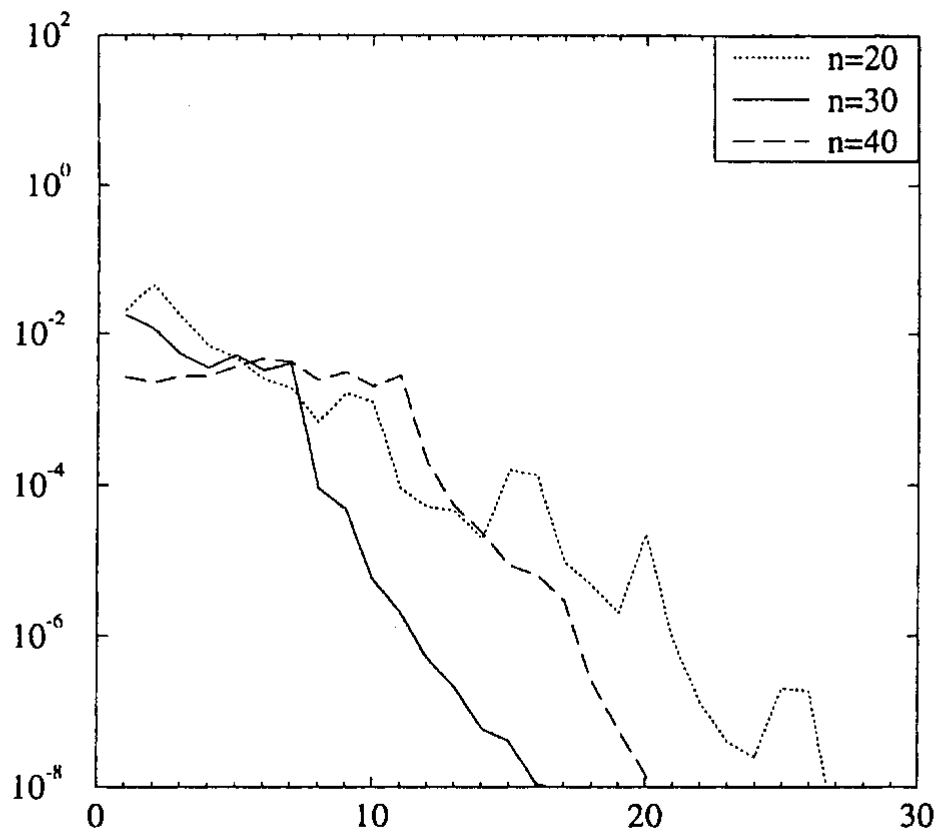
\includegraphics[width=.515\paperwidth]{images/fig-8-5-1.png}
  \caption{\(\varepsilon=10^{-2}\) 时 Galerkin 法在不同网格尺寸下的收敛过程}\label{fig:8.5.1}
\end{figure}
\begin{figure}[!htbp]
  \centering
  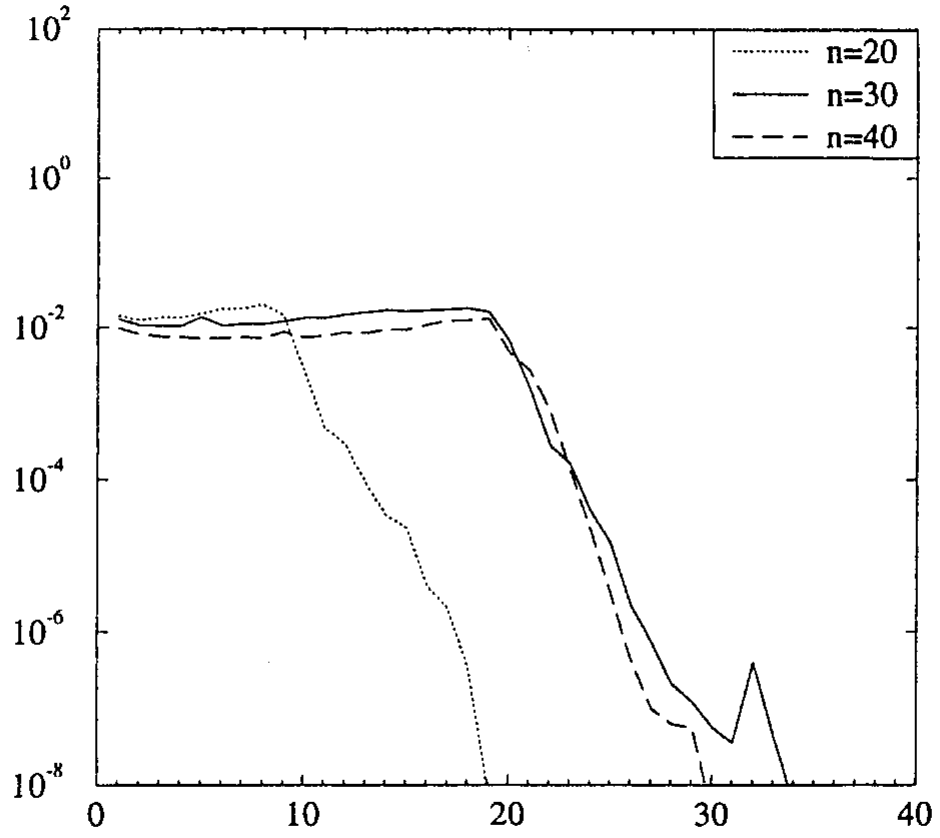
\includegraphics[width=.513\paperwidth]{images/fig-8-5-2.png}
  \caption{\(\varepsilon=10^{-2}\) 时 GALS 法在不同网格尺寸下的收敛过程}\label{fig:8.5.2}
\end{figure}
\begin{figure}[!htbp]
  \centering
  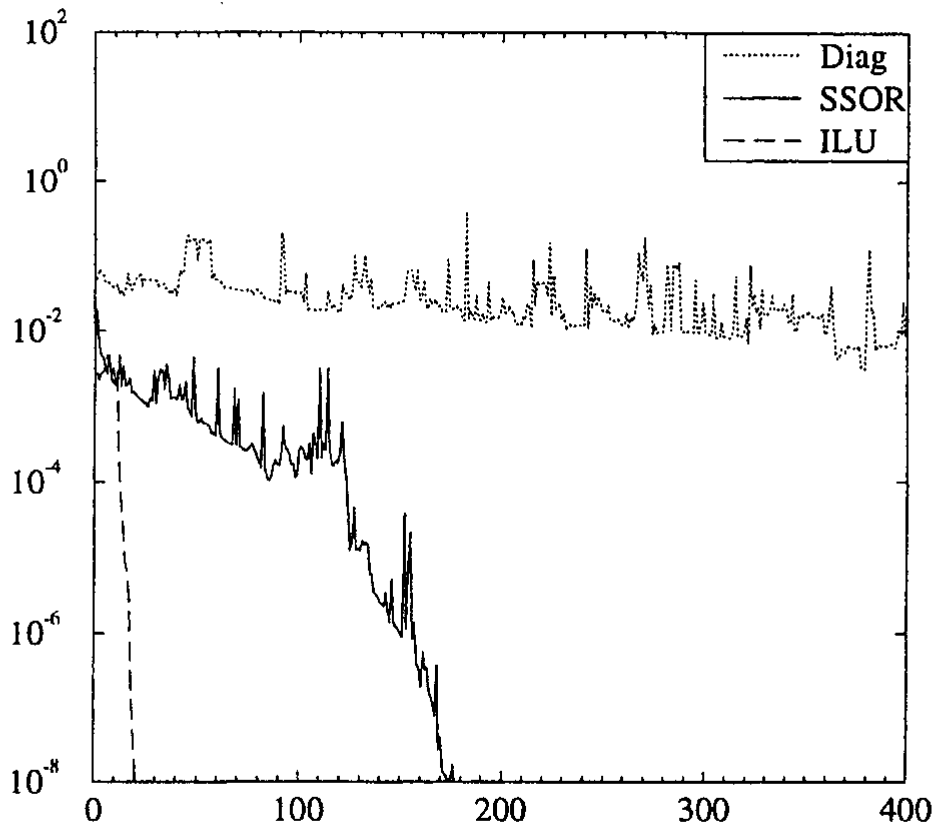
\includegraphics[width=.514\paperwidth]{images/fig-8-5-3.png}
  \caption{\(\varepsilon=10^{-3}\)、\(n=40\) 时 Galerkin 法使用不同预条件矩阵的收敛过程}\label{fig:8.5.3}
\end{figure}
\begin{figure}[!htbp]
  \centering
  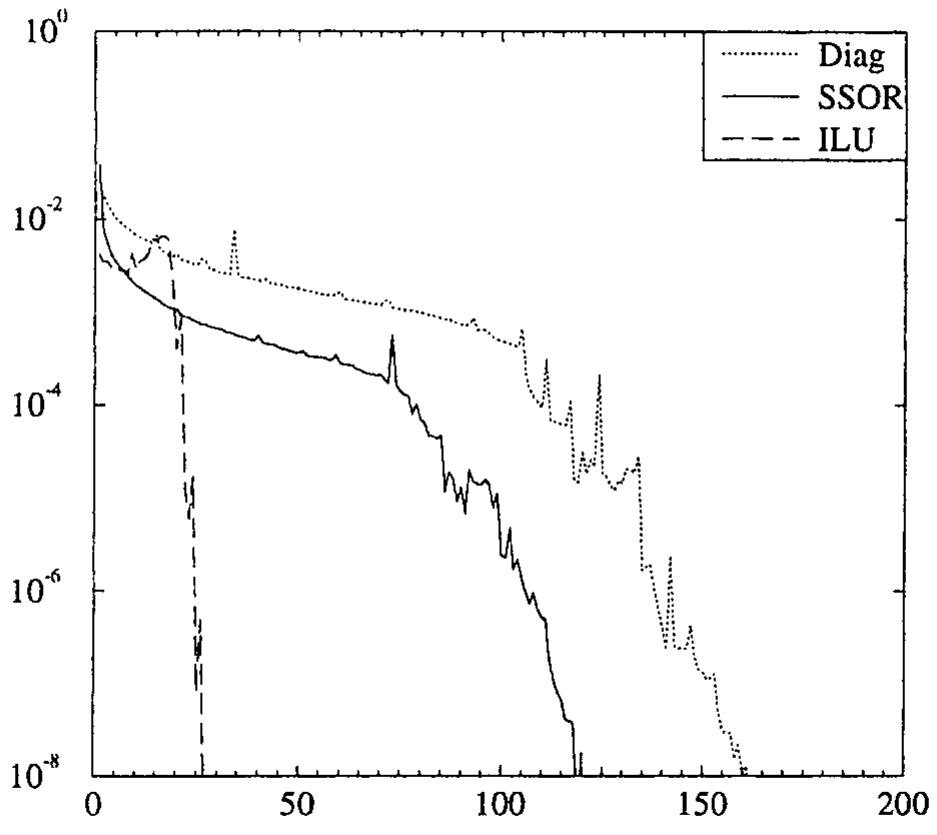
\includegraphics[width=.511\paperwidth]{images/fig-8-5-4.png}
  \caption{\(\varepsilon=10^{-3}\)、\(n=40\) 时 GALS 法使用不同预条件矩阵的收敛过程}\label{fig:8.5.4}
\end{figure}
\begin{figure}[!htbp]
  \centering
  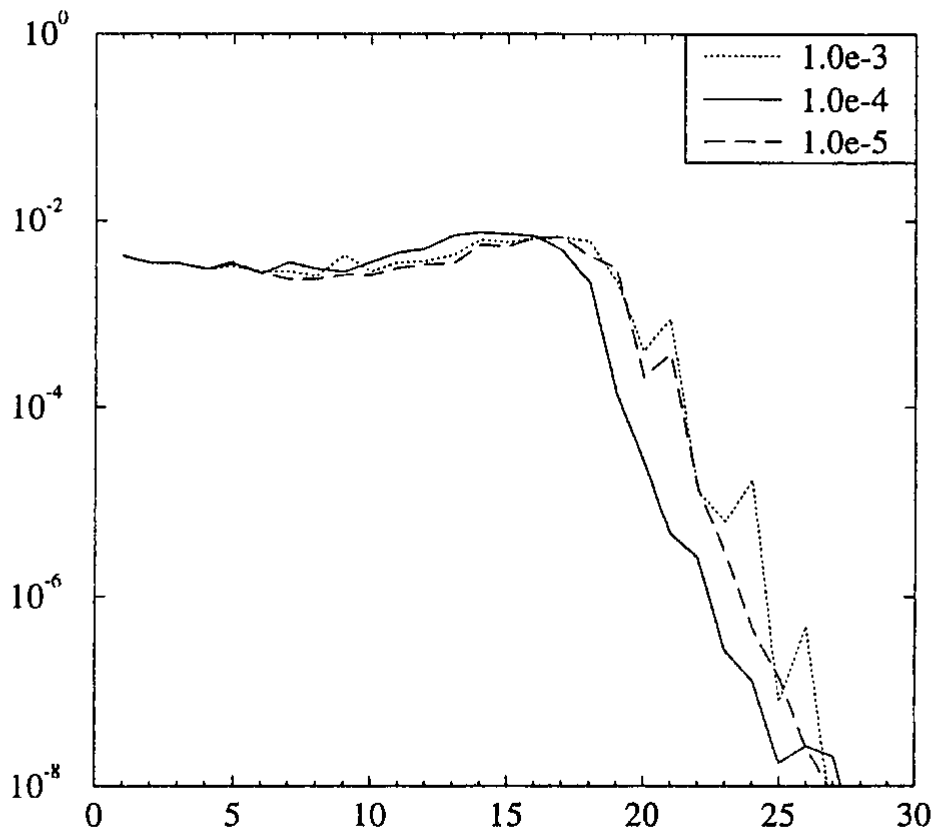
\includegraphics[width=.514\paperwidth]{images/fig-8-5-5.png}
  \caption{\(n=40\) 时 GALS 法对不同 \(\varepsilon\) 的收敛过程}\label{fig:8.5.5}
\end{figure}

\clearpage
\section{异质方法}\label{sec:8.6}
\SourcePage{299}

这里考察另一种方法,可用来逼近形如\eqref{eq:8.3.1}的对流占优的对流--扩散问题.

具体来说,假设\eqref{eq:8.3.1}对应的算子 \(L\) 由\eqref{eq:8.1.1}给出,将它改写为
\[
  Lz=L_1z+L_2z,
\]
其中
\begin{align}
  L_2z&:=-\sum_{i,j=1}^d D_i(a_{ij}D_jz),\label{eq:8.6.1}\\
  L_1z&:=\sum_{i=1}^d D_i(b_iz)+a_0z.\label{eq:8.6.2}
\end{align}
假设\eqref{eq:8.3.12}中定义的函数 \(\alpha_0(\boldsymbol{x})\) 满足
\begin{equation}\label{eq:8.6.3}
  0<\alpha_0\le\alpha_0(\boldsymbol{x})\le\alpha^*
      \qquad\text{在 }\Omega\text{ 上几乎处处},
\end{equation}
且\eqref{eq:6.1.20}成立,使得 \(L\) 对应的双线性形式 \(a(\cdot,\cdot)\) 在 \(H_0^1(\Omega)\) 上具有强制性.此外,假定常数 \(\alpha^*\) 与 \(\boldsymbol{b}\) 的大小相比很小,即
\SourcePage{300}
\[
  \widehat\alpha:=\frac{\alpha^*}{\|\boldsymbol{b}\|_{L^\infty(\Omega)}}\ll1.
\]
因此,可以预期出现边界层或内部层,宽度分别与 \(\widehat\alpha\) 或 \(\sqrt{\widehat\alpha}\) 成正比.

为明确起见,集中讨论边界层.若大致知道边界层的位置(实际中常常如此),就可以只在层的邻域内使用完整算子 \(L\),因为依赖于 \(\alpha_0(\boldsymbol{x})\) 的扩散项只有在那里才有显著影响.在其余区域,可以用\emph{简化算子} \(L_1\) 代替 \(L\),略去黏性的贡献.

\(L_1\) 是一个一阶双曲型算子,属于第~\BookRef{ch:14}{14}~章考察的算子族.这里只指出,在若干情形下,求解双曲型问题 \(L_1u=f\) 的计算量小于求解完整问题 \(Lu=f\) 的计算量.此外,在远离边界层的地方,双曲型问题通常可以用粗网格求解而不影响精度,从而只需在陡峭层附近使用细网格.

显然,这种方法要求将计算区域 \(\Omega\) 分为两个互不相交的区域 \(\Omega_1\) 和 \(\Omega_2\),使 \(\Omega_1\cap\Omega_2=\varnothing\) 且 \(\overline\Omega_1\cup\overline\Omega_2=\overline\Omega\).因此,需要在界面 \(\Gamma:=\partial\Omega_1\cap\partial\Omega_2\) 上对 \(\Omega_2\) 中完整问题的解和 \(\Omega_1\) 中简化问题的解施加适当的匹配条件.

\SourcePage{301}为简便起见,仅讨论齐次 Dirichlet 问题\eqref{eq:8.3.1}.\BookCite{gastaldi-quarteroni-sacchilandriani1990}{Gastaldi、Quarteroni 和 Sacchi Landriani(1990)}提出了下列\emph{耦合问题}：
\begin{equation}\label{eq:8.6.4}
  \begin{cases}
    Lu_2=f,&\text{在 }\Omega_2\text{ 内},\\
    L_1u_1=f,&\text{在 }\Omega_1\text{ 内},\\
    u_2=u_1,&\text{在 }\Gamma^{\mathrm{in}}\text{ 上},\\
    \dfrac{\partial u_2}{\partial n_L}=-\boldsymbol{b}\cdot\boldsymbol{n}\,u_1,
          &\text{在 }\Gamma\text{ 上},\\
    u_2=0,&\text{在 }\partial\Omega_2\cap\partial\Omega\text{ 上},\\
    u_1=0,&\text{在 }\partial\Omega_1^{\mathrm{in}}\cap\partial\Omega\text{ 上},
  \end{cases}
\end{equation}
其中 \(\boldsymbol{n}=\boldsymbol{n}(\boldsymbol{x})\) 是 \(\partial\Omega_1\) 上的单位外法向量,\(\partial u_2/\partial n_L\) 表示 \(u_2\) 关于 \(\boldsymbol{n}\) 的余法向导数,即
\[
  \frac{\partial u_2}{\partial n_L}
     :=\sum_{i,j=1}^d a_{ij}D_ju_2\,n_i-\boldsymbol{b}\cdot\boldsymbol{n}\,u_2.
\]
最后,
\[
  \partial\Omega_1^{\mathrm{in}}
    :=\{\boldsymbol{x}\in\partial\Omega_1\mid \boldsymbol{b}(\boldsymbol{x})\cdot\boldsymbol{n}(\boldsymbol{x})<0\}
\]
\SourcePage{302}是区域 \(\Omega_1\) 的流入边界,并且 \(\Gamma^{\mathrm{in}}:=\partial\Omega_1^{\mathrm{in}}\cap\Gamma\),见\figref{fig:8.6.1}.

匹配条件\eqref{eq:8.6.4}中的第三个条件要求解只在 \(\Gamma^{\mathrm{in}}\) 上连续,第四个条件则在整个界面 \(\Gamma\) 上保证通量平衡.

耦合问题\eqref{eq:8.6.4}可看作求解完整方程\eqref{eq:8.3.1}的一种区域分解表述(见笔记~\ref{note:6.4.1}).由于两侧使用不同的算子,这类方法称为\emph{异质区域分解法},例如见\BookCite{quarteroni-pasquarelli-valli1992}{Quarteroni、Pasquarelli 和 Valli(1992)}.

注意,\eqref{eq:8.6.4}中的界面条件是下面完全椭圆型问题的界面条件所趋向的极限：
\begin{equation}\label{eq:8.6.5}
  L_\varepsilon u_\varepsilon=f\qquad\text{在 }\Omega\text{ 内},
\end{equation}
其中 \(\varepsilon>0\),
\begin{equation}\label{eq:8.6.6}
  L_\varepsilon z:=-\sum_{i,j=1}^d D_i(a_{ij}^\varepsilon D_jz)
     +\sum_{i=1}^d D_i(b_iz)+a_0z,
\end{equation}
并且
\begin{equation}\label{eq:8.6.7}
  a_{ij}^\varepsilon(\boldsymbol{x}):=
  \begin{cases}
    a_{ij}(\boldsymbol{x}),&\boldsymbol{x}\in\Omega_2,\\
    \varepsilon\delta_{ij},&\boldsymbol{x}\in\Omega_1.
  \end{cases}
\end{equation}
事实上,这时 \(L_\varepsilon u_\varepsilon=f\) 在 \(\Omega\) 内的解 \(u_\varepsilon\) 在 \(\Gamma\) 上满足
\SourcePage{303}
\begin{figure}[!htbp]
  \centering
  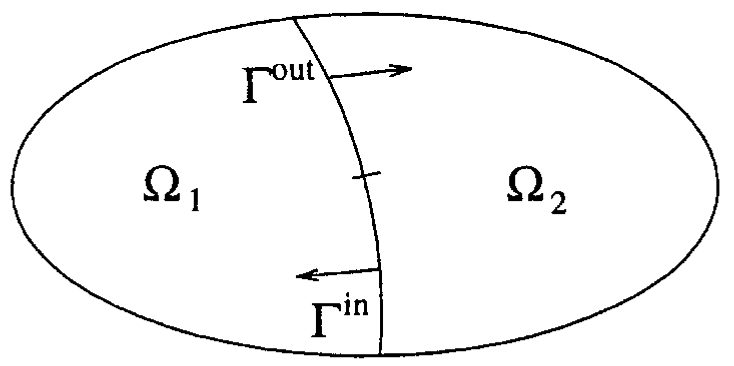
\includegraphics[width=.400\paperwidth]{images/fig-8-6-1.png}
  \caption{区域 \(\Omega\) 的分解}\label{fig:8.6.1}
\end{figure}
\begin{equation}\label{eq:8.6.8}
  \begin{cases}
    u_\varepsilon|_{\Omega_2}=u_\varepsilon|_{\Omega_1},\\
    \dfrac{\partial(u_\varepsilon|_{\Omega_2})}{\partial n_L}
       =\varepsilon\dfrac{\partial(u_\varepsilon|_{\Omega_1})}{\partial n}
         -\boldsymbol{b}\cdot\boldsymbol{n}\,u_\varepsilon|_{\Omega_1}.
  \end{cases}
\end{equation}
在取极限的过程中,解的连续性只在 \(\Gamma^{\mathrm{in}}\) 上保留.不过,可以证明,\(\Gamma\setminus\Gamma^{\mathrm{in}}\) 上的跳跃幅度与 \(\max_\Gamma\alpha_0(\boldsymbol{x})\) 一样小.

现在讨论\eqref{eq:8.6.4}的有限维逼近.先引入双线性形式
\begin{equation}\label{eq:8.6.9}
  a_2(z,v):=\int_{\Omega_2}
    \left[\sum_{i,j=1}^d a_{ij}D_jzD_iv-\sum_{i=1}^d b_izD_iv+a_0zv\right]
\end{equation}
\SourcePage{304}
及
\begin{equation}\label{eq:8.6.10}
  a_1(z,v):=\int_{\Omega_1}\left[-\sum_{i=1}^d b_izD_iv+a_0zv\right].
\end{equation}
于是,将\eqref{eq:8.6.4}改写为：求 \(u_2\in H^1_{\partial\Omega_2\setminus\Gamma}(\Omega_2)\)、\(u_1\in L^2(\Omega_1)\),使
\begin{equation}\label{eq:8.6.11}
  \left\{
  \begin{aligned}
    &a_2(u_2,v_2)-(\boldsymbol{b}\cdot\boldsymbol{n}\,u_2,v_2)_{\Gamma^{\mathrm{in}}}\\
    &\quad=(f,v_2)_{\Omega_2}+(\boldsymbol{b}\cdot\boldsymbol{n}\,u_1,v_2)_{\Gamma^{\mathrm{out}}}
         \qquad\forall\,v_2\in H^1_{\partial\Omega_2\setminus\Gamma}(\Omega_2),\\
    &a_1(u_1,v_1)+(\boldsymbol{b}\cdot\boldsymbol{n}\,u_1,v_1)_{\partial\Omega_1^{\mathrm{out}}}\\
    &\quad=(f,v_1)_{\Omega_1}-(\boldsymbol{b}\cdot\boldsymbol{n}\,u_2,v_1)_{\Gamma^{\mathrm{in}}}
          \qquad\forall\,v_1\in H^1(\Omega_1),
  \end{aligned}
  \right.
\end{equation}
其中 \(\Gamma^{\mathrm{out}}:=\Gamma\setminus\Gamma^{\mathrm{in}}\)、\(\partial\Omega_1^{\mathrm{out}}:=\partial\Omega_1\setminus\partial\Omega_1^{\mathrm{in}}\),并且
\[
  H^1_{\partial\Omega_2\setminus\Gamma}(\Omega_2)
      :=\{v\in H^1(\Omega_2)\mid v=0\text{ 在 }\partial\Omega_2\setminus\Gamma\text{ 上}\}
\]
(见第~\ref{sec:1.3}~节).在涉及 \(u_1\) 的边界项中,用 \(\boldsymbol{b}u_1\) 的法向迹解释其通量.

注意,\eqref{eq:8.6.11}的第一个方程保证\eqref{eq:8.6.4}中的第一个方程成立,此外还给出
\begin{align}
  \sum_{i,j=1}^d a_{ij}(D_ju_2)n_i&=0
    &&\text{在 }\Gamma^{\mathrm{in}}\text{ 上},\label{eq:8.6.12}\\
  \frac{\partial u_2}{\partial n_L}&=-\boldsymbol{b}\cdot\boldsymbol{n}\,u_1
    &&\text{在 }\Gamma^{\mathrm{out}}\text{ 上}.\label{eq:8.6.13}
\end{align}
而\eqref{eq:8.6.11}的第二个方程蕴含\eqref{eq:8.6.4}的第二个方程以及
\begin{equation}\label{eq:8.6.14}
  u_1=u_2\qquad\text{在 }\Gamma^{\mathrm{in}}\text{ 上}.
\end{equation}
界面条件\eqref{eq:8.6.12}至\eqref{eq:8.6.14}显然等价于\eqref{eq:8.6.4}的第三个和第四个条件.

还应注意,从\eqref{eq:8.6.11}的第二个方程可知,\(u_1\) 确实满足 \(\operatorname{div}(\boldsymbol{b}u_1)\in L^2(\Omega_1)\),所以 \(\partial\Omega_1\) 上的迹 \(\boldsymbol{b}\cdot\boldsymbol{n}\,u_1\) 有明确定义(见定理~\ref{thm:1.3.2}).

可以通过逐子域迭代有效地求解\eqref{eq:8.6.11},交替地在各自的区域内求解双曲型方程和椭圆型方程.这种策略便于数值计算,因为两个区域可以采用不同的求解器,甚至可以采用不同的空间离散.

下面给出\eqref{eq:8.6.11}基于 Galerkin 法的有限维逼近.设 \(V_{2,h}\) 和 \(V_{1,h}\) 分别为 \(H^1_{\partial\Omega_2\setminus\Gamma}(\Omega_2)\) 和 \(H^1(\Omega_1)\) 的适当有限维子空间.离散问题写成：求 \(u_{2,h}\in V_{2,h}\)、\(u_{1,h}\in V_{1,h}\),使
\SourcePage{305}
\begin{equation}\label{eq:8.6.15}
  \left\{
  \begin{aligned}
    &a_2(u_{2,h},v_{2,h})-(\boldsymbol{b}\cdot\boldsymbol{n}\,u_{2,h},v_{2,h})_{\Gamma^{\mathrm{in}}}\\
    &\quad=(f,v_{2,h})_{\Omega_2}+(\boldsymbol{b}\cdot\boldsymbol{n}\,u_{1,h},v_{2,h})_{\Gamma^{\mathrm{out}}}
         \qquad\forall\,v_{2,h}\in V_{2,h},\\
    &a_1(u_{1,h},v_{1,h})+(\boldsymbol{b}\cdot\boldsymbol{n}\,u_{1,h},v_{1,h})_{\partial\Omega_1^{\mathrm{out}}}\\
    &\quad=(f,v_{1,h})_{\Omega_1}-(\boldsymbol{b}\cdot\boldsymbol{n}\,u_{2,h},v_{1,h})_{\Gamma^{\mathrm{in}}}
         \qquad\forall\,v_{1,h}\in V_{1,h}.
  \end{aligned}
  \right.
\end{equation}
求解这一问题的一种有效迭代方法如下.给定任意初始近似 \(u_{2,h}^0\in V_{2,h}\),对 \(k\ge1\) 先求解
\begin{equation}\label{eq:8.6.16}
  \begin{aligned}
    &a_1(u_{1,h}^k,v_{1,h})+(\boldsymbol{b}\cdot\boldsymbol{n}\,u_{1,h}^k,v_{1,h})_{\partial\Omega_1^{\mathrm{out}}}\\
    &\quad=(f,v_{1,h})_{\Omega_1}-(\boldsymbol{b}\cdot\boldsymbol{n}\,u_{2,h}^{k-1},v_{1,h})_{\Gamma^{\mathrm{in}}}
         \qquad\forall\,v_{1,h}\in V_{1,h},
  \end{aligned}
\end{equation}
再求解
\begin{equation}\label{eq:8.6.17}
  \begin{aligned}
    &a_2(u_{2,h}^k,v_{2,h})-(\boldsymbol{b}\cdot\boldsymbol{n}\,u_{2,h}^k,v_{2,h})_{\Gamma^{\mathrm{in}}}\\
    &\quad=(f,v_{2,h})_{\Omega_2}+(\boldsymbol{b}\cdot\boldsymbol{n}\,u_{1,h}^k,v_{2,h})_{\Gamma^{\mathrm{out}}}
         \qquad\forall\,v_{2,h}\in V_{2,h}.
  \end{aligned}
\end{equation}
这两个问题都可求解,因为相应的矩阵正定.

\begin{figure}[!htbp]
  \centering
  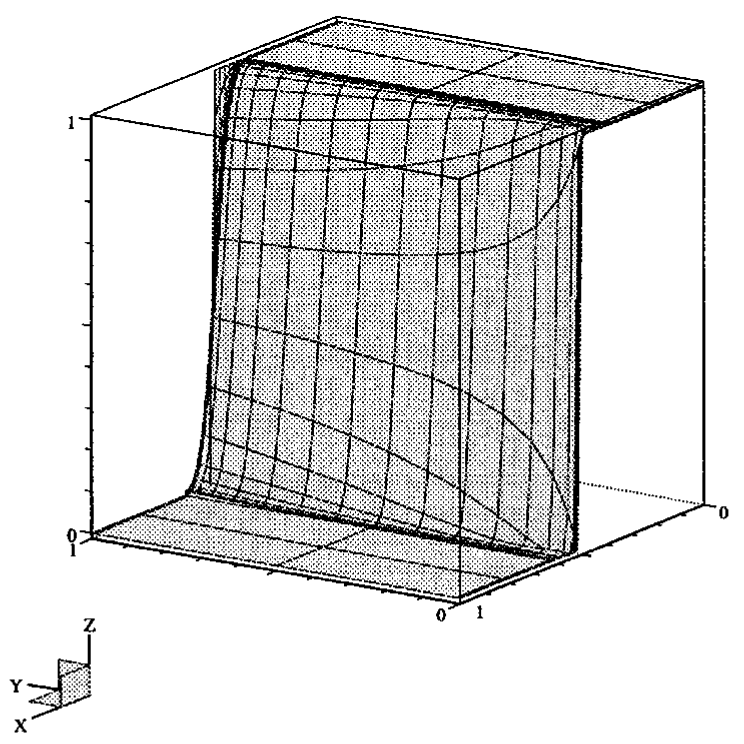
\includegraphics[width=.406\paperwidth]{images/fig-8-6-2.png}
  \caption{用异质方法为具有一个内部层的第一个测试问题计算的数值解}\label{fig:8.6.2}
\end{figure}

在二维情形,\BookCite{gastaldi-quarteroni-sacchilandriani1990}{Gastaldi、Quarteroni 和 Sacchi Landriani(1990)}证明了采用谱配置法时这一迭代格式的收敛性,且收敛速率与离散参数 \(h\) 无关.\SourcePage{306}也可使用加速参数 \(\theta_k>0\),将\eqref{eq:8.6.16}右端的 \(u_{2,h}^{k-1}\) 替换为 \(\lambda_h^{k-1}:=\theta_ku_{2,h}^{k-1}+(1-\theta_k)u_{1,h}^{k-1}\),这里还需要另选一个初值 \(u_{1,h}^0\in V_{1,h}\).

关于这一方法实际表现的全面介绍,见\BookCite{quarteroni-pasquarelli-valli1992}{Quarteroni、Pasquarelli 和 Valli(1992)}及\BookCite{frati-pasquarelli-quarteroni1993}{Frati、Pasquarelli 和 Quarteroni(1993)}.

\BookCite{brezzi-canuto-russo1989}{Brezzi、Canuto 和 Russo(1989)}提出了另一种处理椭圆型与双曲型耦合的方法,称为 \(\chi\) 表述,亦见\BookCite{canuto-russo1993}{Canuto 和 Russo(1993)}及其中所引文献.

下面给出两个用异质方法得到的数值结果,其中将 \(\Omega\subset\mathbb R^2\) 划分成两个以上的子区域.\figref{fig:8.6.2}是\figref{fig:8.3.3}\subref{fig:8.3.3a}的对应结果.将 \(\Omega\) 划分成九个子区域,只在含有内部层的三个子区域中求解完整的椭圆型问题(\(\varepsilon=10^{-3}\)),其余各子区域令 \(\varepsilon=0\).用 Legendre 谱配置法计算数值解,总共采用 874 个配置点.

\figref{fig:8.6.3}对应对流场 \(\boldsymbol{b}=(x_1,x_2)\)、\(\varepsilon=10^{-4}\) 的情形.将 \(\Omega\) 划分成九个子区域：一个较大的内部“双曲型”子区域和八个紧邻边界的狭长子区域.在后八个子区域中求解完整的椭圆型问题.“双曲型”子区域采用 9 个配置点,每个角部子区域采用 49 个,其余四个“边界”子区域各采用 21 个.

\begin{figure}[!htbp]
  \centering
  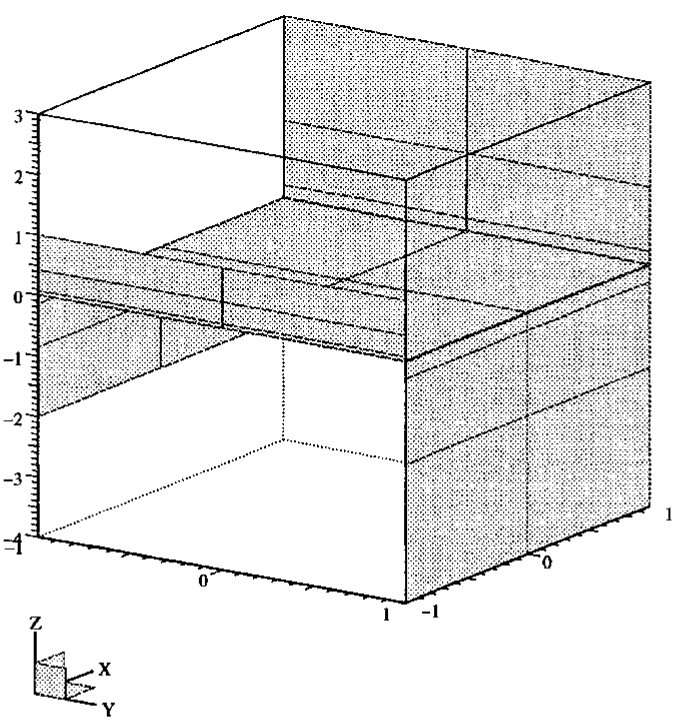
\includegraphics[width=.372\paperwidth]{images/fig-8-6-3.png}
  \caption{用异质方法为具有四个边界层的第二个测试问题计算的数值解}\label{fig:8.6.3}
\end{figure}
